\section{Results and interpretation}
\label{sec:results}

\subsection{Statistical approach}

\subsubsection{The modified frequentist approach: asymptotic formulae to extract an upper limit on signal strength}

The modified frequentist approach, also known as $CL_s$ criterion~\cite{bib:CLS1,bib:CLS2,bib:LHC-HCG-Report}, is used to determine the 95\% confidence level upper limit on the signal contribution in the data.%, using the {\tt RooStats} package~\cite{Moneta:2010pm}.
%In order to extract the limit on the production cross-section times the branching ratios, the CMS standard {\tt combine} tool~\cite{bib:combine} has been used.

\noindent The parameters used to model the data distribution are the background event yield, $b$, the signal event yield $s$, predicted by the theoretical model, the signal strength modifier $\mu$, parametrizing how much the signal yield deviates from the model expectation $s$, and the nuisance parameters $\theta$, namely, the uncertainties affecting the signal and background yields, that can be seen as functions of the nuisances: $b(\theta)$, $s(\theta)$. In this approach, the uncertainties are considered either as fully correlated (100\%) or uncorrelated.

\noindent The likelihood function is built starting from a Poissonian probability density function:
\begin{equation}
%\mathbb{L} 
\mathfrak{L} (\text{ data }| \mu, \theta) = \text{Poisson } (\text{ data } | \mu \cdot s(\theta) + b(\theta)) \cdot p (\tilde{\theta}| \theta),
\label{eq:likelihood}
\end{equation}
where ``data'' can either be real or generated pseudo-data, whilst $p (\tilde{\theta}| \theta)$ is the probability distribution of the nuisance parameters, inferred through an independent dataset $\tilde{\theta}$. Considering an unbinned likelihood, where $k$ events have been observed,
\begin{equation}
%\mathbb{L} 
\text{Poisson } (\text{ data } | \mu \cdot s(\theta) + b(\theta)) = \frac{1}{k} \prod_i \left( \mu S f_s(x_i) + B f_b (x_i) \right) \times e^{- (\mu S + B)},
\end{equation}
where $f_s$ and $f_b$ are the probability density functions for signal and background for an observable $x$, and $S$ and $B$ are the total expected signal and background event yields.

\noindent The measurement of the compatibility of data with the signal plus background or the background-only hypotheses is performed by defining a likelihood ratio test statistics $\tilde{q}_{\mu}$~\cite{bib:Asymptotic},
\begin{equation}
\begin{gathered}
\tilde{q}_{\mu} = -2 \log { \frac{\mathfrak{L} (\text{data }| \mu, \hat{\theta}_{\mu}) }{ \mathfrak{L} (\text{data }| \hat{\mu}, \hat{\theta})  } },\\
0 \leq \hat{\mu} \leq \mu.
\end{gathered}
\end{equation}

\noindent The quantities $\hat{\mu}$ and $\hat{\theta}$ are global maxima of the likelihood, while $\hat{\theta}_{\mu}$ is the conditional maximum, given $\mu$. The signal strength $\hat{\mu}$ is defined positive, the upper boundary $\hat{\mu} \leq \mu$ is set in order to avoid to consider upward fluctuations in data (namely, when the global maximum is larger than the hypothesis $\mu$) as an incompatibility with the signal hypothesis ($\mu$).

\noindent Given the $\mu$ hypothesis, the test statistic value is measured on data, and labelled as $\tilde{q}_{\mu}^{\text{obs.}}$. Parameters $\hat{\theta}_0^{\text{obs.}}$ and $\hat{\theta}_{\mu}^{\text{obs.}}$ are calculated by maximizing the likelihood function~\ref{eq:likelihood}. Toy Monte Carlo pseudo-data are then generated to build the probability density functions $f(\tilde{q}_{\mu}|\mu, \hat{\theta}_{\mu}^{\text{obs.}})$ (signal with $\mu$ strength hypothesis) and $f(\tilde{q}_{\mu}|0, \hat{\theta}_0^{\text{obs.}})$ (background-only hypothesis). Nuisance parameters are fixed to their values measured on data, $\hat{\theta}_{\mu}^{\text{obs.}}$ and $\hat{\theta}_0^{\text{obs.}}$, but left free to float in fits that are required to evaluate $\tilde{q}_{\mu}$.

\noindent The p-values associated to signal plus background and background-only hypotheses are defined as:
\begin{equation}
\begin{gathered}
p_{\mu} = \mathcal{P} \left( \tilde{q}_{\mu} \geq \tilde{q}_{\mu}^{\text{obs.}} | \text{ signal + background } \right) = \int_{\tilde{q}_{\mu}^{\text{obs.}}}^{\infty} f(\tilde{q}_{\mu}|\mu, \hat{\theta}_{\mu}^{\text{obs.}}) d \tilde{q}_{\mu} ,\\
1 - p_b = \mathcal{P} \left( \tilde{q}_{\mu} \geq \tilde{q}_{\mu}^{\text{obs.}} | \text{ background-only } \right) = \int_{\tilde{q}_{\mu}^{\text{obs.}}}^{\infty} f(\tilde{q}_{\mu}|0, \hat{\theta}_{0}^{\text{obs.}}) d \tilde{q}_{\mu} .\\
\end{gathered}
\end{equation}

\noindent The $CL_s$ is defined as the ratio of the above p-values:

\begin{equation}
CL_s = \frac{ p_{\mu} }{ 1 - p_b}.
\end{equation}

\noindent Given the a-priori confidence level $\alpha$, if $CL_s \leq \alpha$, a model with signal strength $\mu$ is excluded at $(1 - \alpha)$ confidence level (C.L.). The 95\% C.L. \emph{observed} upper limit on the theoretical model is set by extracing $\mu$ from the equation $CL_s = 0.05$.

\noindent Similarly to the observed limit, an upper \emph{expected} limit, along with the $\pm 1 \sigma$ and $\pm 2 \sigma$ uncertainty bands, can be extracted by generating pseudo-data under the background-only hypothesis, and by calculating the $CL_s$ and 95\% upper limit for each of the pseudo-data. A cumulative distribution of the calculated upper limits is then constructed: the 50\% quantile corresponds to the median expected, the 2.5\%, 16\%, 84\%, 95.5\% quantiles correspond respectively to $-2 \sigma$, $-1 \sigma$, $+1 \sigma$, $+2 \sigma$ uncertainty bands.

\noindent Generating a large number of pseudo-data, however, can be a very expensive computational effort. This problem is overcome by profiting of asymptotic formulae~\cite{bib:Asymptotic}, derived through Wilk's~\cite{bib:Wilks} and Wald's~\cite{10.2307/1990256} theorems. The set of pseudo-data is replaced by only one dataset, the Asimov dataset: it corresponds to a dataset where the statistical fluctuations are suppressed, and hence every parameter is set to its expectation value. These values are then equivalent to the outcomes of a large sample of Monte Carlo simulations. The \emph{expected} limit can therefore be calculated from the Asimov dataset.

\noindent By using the asymptotic formulae, the distribution of the test statistic $\tilde{q}_{\mu}$ is given by:
\begin{equation}
\begin{gathered}
f(\tilde{q}_{\mu}|\mu) = \frac{1}{2} \delta (\tilde{q}_{\mu}) + 
\left\{
\begin{array}{l}
\begin{gathered}
\frac{1}{2 \sqrt{2 \pi}} \frac{1}{\tilde{q}_{\mu}} e^{-\tilde{q}_{\mu}/2} \text{ \hspace*{1.8cm}} 0 < \tilde{q}_{\mu} \leq \mu^2 / \sigma^2\\
\frac{1}{2 \sqrt{2 \pi}} \frac{1}{2 \mu / \sigma} e^ {-\frac{1}{2} \frac{\left(\tilde{q}_{\mu}  + \mu^2 / \sigma^2 \right)^2}{\left( 2 \mu / \sigma \right)^2}  } \text{ \hspace*{0.5cm}  } \tilde{q}_{\mu} > \mu^2 / \sigma^2\\
\end{gathered}
\end{array}
\right. ; \\
\sigma^2 = \frac{\mu^2}{ \tilde{q}_{\mu, A}},
\end{gathered}
\end{equation}

\noindent where the test statistic $\tilde{q}_{\mu, A}$ is evaluated in the Asimov dataset. Once defined $\Phi$, the inverse of the cumulative Gaussian distribution, the asymptotic expression of the $CL_s$ simplifies into:
\begin{equation}
CL_s = \frac{1 - \Phi \left( \sqrt{\tilde{q}_{\mu}} \right)}{ \Phi \left( \sqrt{\tilde{q}_{\mu, A}} - \sqrt{\tilde{q}_{\mu}} \right) }.
\end{equation}

\noindent The expected upper limit and its $N$ uncertainty bands are given by:
\begin{equation}
\begin{gathered}
\mu_{up} = \sigma \cdot \Phi^{-1} \left( 1 - 0.5 \alpha \right),\\
\mu_{up + N} = \sigma \cdot \left[ \Phi^{-1}  \left( 1 - \alpha \Phi(N)  \right) + N \right].\\
\end{gathered}
\end{equation}

\subsubsection{Treatment of the systematic uncertainties}
The nuisance parameters $\theta$, introduced to describe the systematic uncertainties, are expected to have their own probability density function, $\rho (\theta)$, called \emph{prior}, that is inferred by an additional set of measurements $\tilde{\theta}$, used to define the mean, the shape and the width of each uncertainty. The distribution of the priors depends on the type of uncertainty considered. Flat priors (namely, a constant value) are assigned to nuisances unconstrained a-priori; Gaussian priors are assigned to nuisances allowed to assume both negative and positive values; log-normal priors are used for positively defined nuisances (such as cross-sections, efficiencies, luminosity, scale factors). For the purpose of this search, log-normal priors are being adopted. Partially correlated uncertainties, \textit{i.e.} those associated to the $\alpha$ method parameters, are decorellated through linear transformations.

\subsubsection{Computation of local p-values}
The discovery of a signal can be inferred from data if a p-value that is incompatible with the background-only hypothesis is observed. The discovery test statistics is defined as:

\begin{equation}
\begin{gathered}
{q}_{0} = -2 \log { \frac{\mathfrak{L} (\text{data }| 0, \hat{\theta_{0}}) }{ \mathfrak{L} (\text{data }| \hat{\mu}, \hat{\theta})  } },\\
\hat{\mu} \geq 0.\\
\end{gathered}
\end{equation}

\noindent The boundary $\hat{\mu} \geq 0$ is motivated by the fact that an underfluctuation of the background is not considered as an evidence against the background-only hypothesis. The distribution $f (q_0 | 0, \hat{\theta}_0^{obs})$ is again built with pseudo-data, generated under the background-only hypothesis with nuisances $\hat{\theta}_0^{obs}$. The exact p-value is therefore:

\begin{equation}
p_0 = \mathcal{P} \left( q_0 \geq q_0^{\text{obs.}} | \text{ background-only } \right) = \int_{q_0^{\text{obs.}}}^{\infty} f (q_0 | 0, \hat{\theta}_0^{obs}) d q_0,
\label{eq:local_pvalue}
\end{equation}

\noindent that can be converted into a significance $Z$, once the convention of the one-sided Gaussian tail is adopted:

\begin{equation}
p_0 = \int_Z^{\infty} \frac{1}{\sqrt{2 \pi}} e^{-x^2/2} dx.
\end{equation} 

\noindent By taking advantage of the Wilk's theorem, the p-value can be approximated as:

\begin{equation}
p_0^{\text{appr.}} = \frac{1}{2} \left[ 1 - \text{Erf } \left( \sqrt{q_0^{\text{obs.}}/2}\right) \right].
\end{equation} 

\noindent Since the p-value depends on the phase-space considered (specifically, on the resonance mass hypothesis), eq.~\ref{eq:local_pvalue} is known as the \emph{local p-value}. A scan of the local p-values is a measurement of a local departure from the background-only hypothesis. In case of a local excess, the global significance is computed by correcting the local significance with trial factors, that take into account the so-called \emph{look-elsewhere} effect~\cite{Gross2010}, namely, the probability to observe the same excess anywhere in the whole mass range.

%{\color{red} Pari pari alla tesi di Alberto:}
%The {\tt Asymptotic} method is used to calculate preliminary 95\% C.L. upper limits with $1 \sigma$ and $2 \sigma$ bands using the CLs frequentist calculation currently recommended by the LHC Higgs Combination Group~\cite{bib:statpaper}. The {\tt ProfileLikelihood} method is used for significance and the background p-value; finally, the {\tt MaxLikelihoodFit} method allows to get the signal Best Fit Ratio, the fit pulls and the pre/post fit distributions.

\subsection{Signal extraction strategy for the analysis}

The background prediction, estimated with the $\alpha$ method (sec.~\ref{sec:alpha}), the signal parametrization (sec.~\ref{ssec:signal_parametrization}), and the observed data are used as inputs for the signal extraction procedure. An unbinned maximum likelihood fit is performed on each purity category, and on the combination of the categories, in order to present, for each theoretical model taken into account, a global limit on the production cross-section times branching fraction, that is the parameter describing the signal yield and defining the signal strength $r$ (equivalent to the signal strength $\mu$ discussed in the previous section).

\subsubsection{Fit diagnostics: nuisances pulls and impacts}

The systematic uncertainties, treated as log-normal nuisance parameters, are allowed to vary around their nominal values and are profiled during the maximum likelihood estimation of the signal strength. As a diagnostic, the profiled values (post-fit) of the nuisance parameters $\hat{\theta}$ are compared to their a-priori expectations (pre-fit) $\theta_0$, in unities of the width of the Gaussian core of the nuisance parameter $\Delta \theta$. The quantities $(\hat{\theta} - \theta_0) / \Delta \theta$ are called \emph{nuisance pulls}, and they have been computed both in the background-only hypothesis (blue bars) and in the signal plus background hypothesis (green bars), for the low- (fig.~\ref{fig:pulls_lp}) and high-purity (fig.~\ref{fig:pulls_hp}) categories. In fig.~\ref{fig:pulls_lp}-\ref{fig:pulls_hp}, the signal of a spin-2 bulk graviton with a mass of 3 \TeV is considered. The distribution of pulls does not show any anomaly, since pulls are centered around zero (no discrepancies with the a-priori expectations) and their widths are around one (no strong deviations from the original assumption on the width of the nuisance distributions), for both the background-only and signal plus background hypotheses. The only pulls with mean values a bit shifted from zero or with widths smaller than one are related to $\alpha$ method parameters, that are under control.

\noindent The \emph{impacts} of a nuisance parameter $\theta$ are defined as the shifts induced in the signal strength ($r$, the cross-section times branching fraction in this case) as $\theta$ is fixed and brought to its +1$\sigma$ or -1$\sigma$ post-fit values, while all the other nuisance parameters are simultaneously profiled as log-normal. In fig.~\ref{fig:impacts}, impacts are calculated by combining the two purity categories, assuming a signal hypothesis of a spin-2 bulk graviton of mass 2.5 \TeV. As expected a-priori (sec.~\ref{sec:uncertainties}), the most relevant systematic uncertianty impacting on the determination of the signal strength is represented by the uncertainty on the \V-tagging procedure. No pathological behaviour can be observed. %extrapolation at high \pt.

\begin{figure}[!h]
   \caption{Nuisance pulls for the low-purity category, calculated under both the background-only (blue bars) and signal plus background hypotheses (green bars). A signal hypothesis of a spin-2 bulk graviton of mass 3 \TeV is considered.}
 \begin{center}
   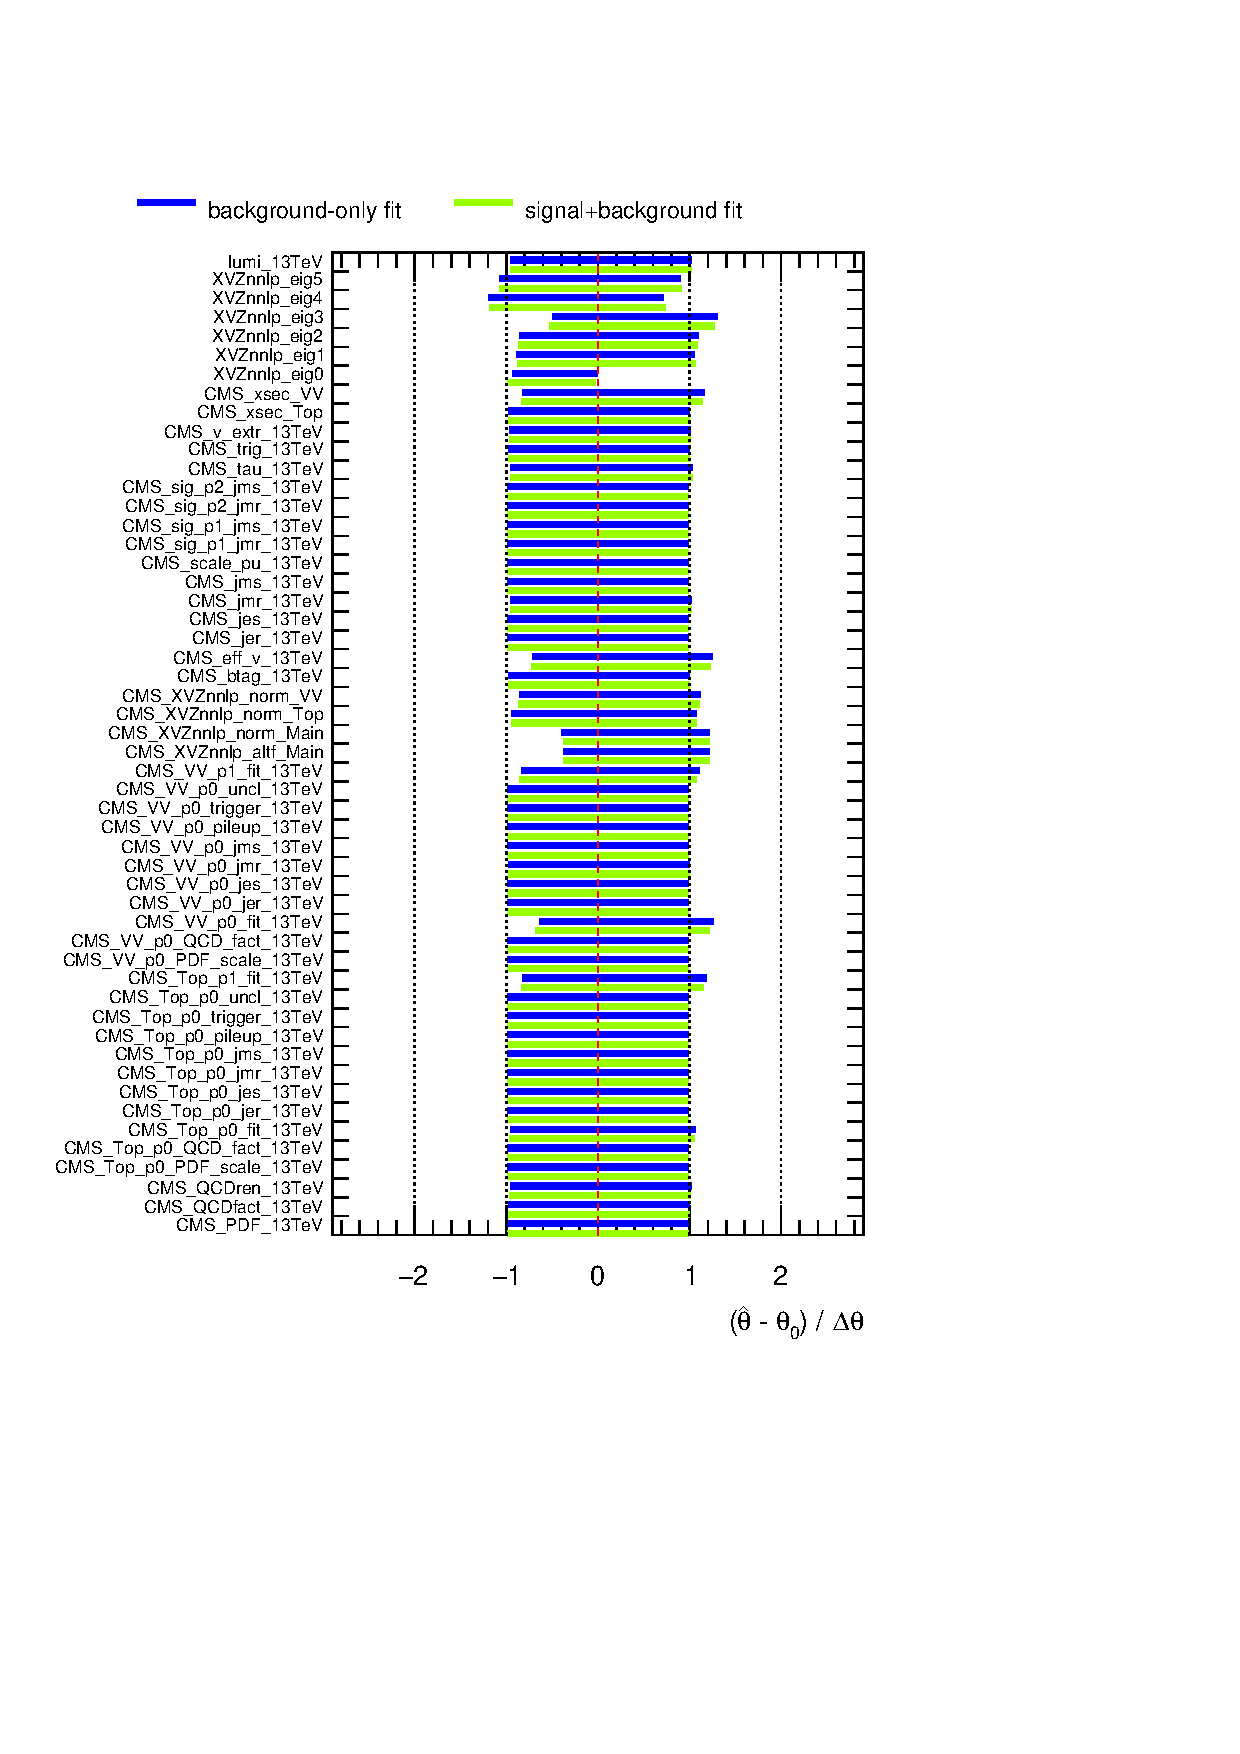
\includegraphics[width=0.8\textwidth]{pulls_VZ_data_1fb/pulls_XZZInv_lp3000.pdf}
   \label{fig:pulls_lp}
 \end{center}
\end{figure}

\begin{figure}[!h]
   \caption{Nuisance pulls for the high-purity category, calculated under both the background-only (blue bars) and signal plus background hypotheses (green bars). A signal hypothesis of a spin-2 bulk graviton of mass 3 \TeV is considered.}
 \begin{center}
   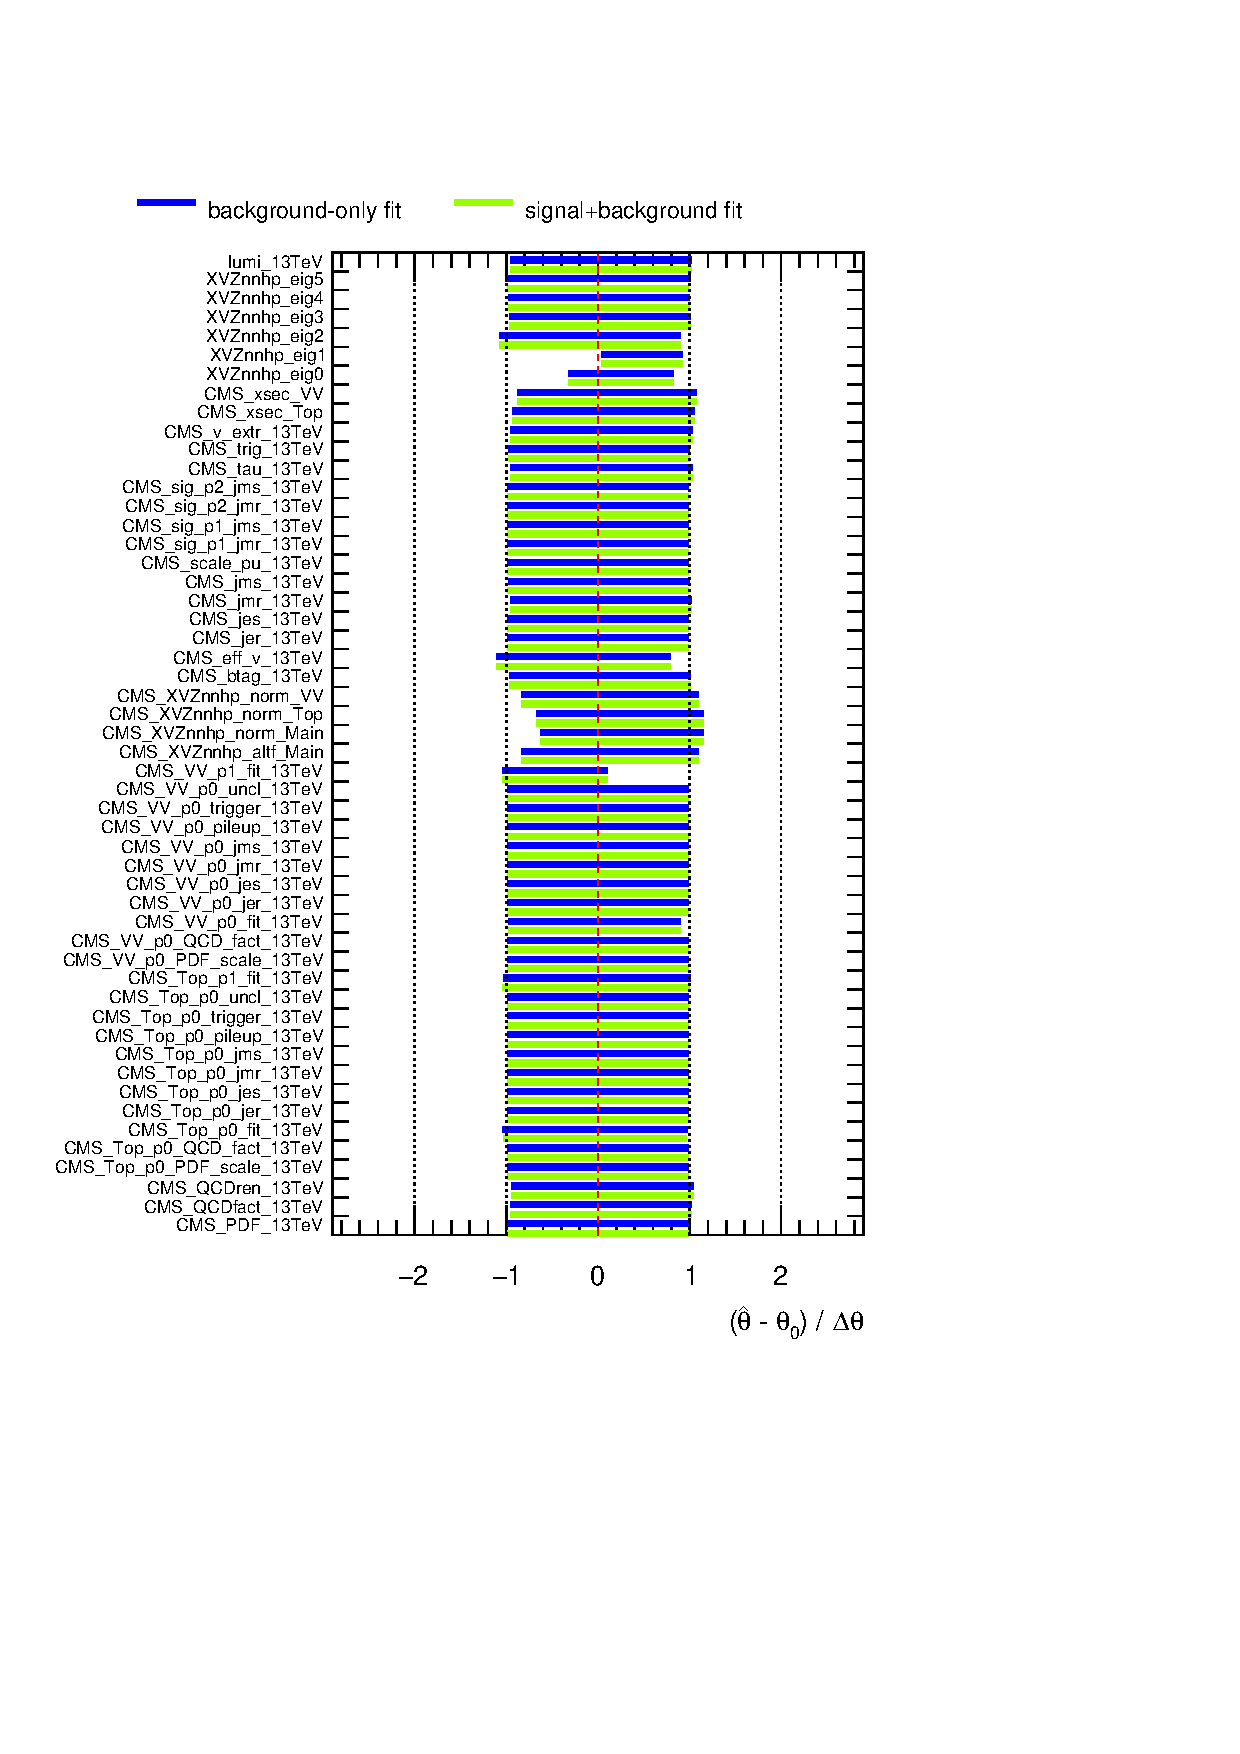
\includegraphics[width=0.8\textwidth]{pulls_VZ_data_1fb/pulls_XZZInv_hp3000.pdf}
   \label{fig:pulls_hp}
 \end{center}
\end{figure}


\begin{figure}[!h]
   \caption{Impacts of the nuisance parameters on the signal strength estimation, for the combination of the low- and high-purity categories. A signal hypothesis of a spin-2 bulk graviton of mass 2.5~\TeV is considered. $\theta_0$ is the pre-fit value of the nuisance parameter taken into account; $\hat{\theta}$ is the value of the nuisance parameter after the maximum likelihood fit; $\Delta \hat{r}$ represents the impact, \textit{i.e.} the shift induced in the parameter of interest (in this case, $r$, the cross-section times branching fraction, describing the signal strength) as the $\theta$ parameter is fixed and brought to its +1$\sigma$ or -1$\sigma$ post-fit values, with all the other nuisance parameters profiled as log-normal.}
 \begin{center}
   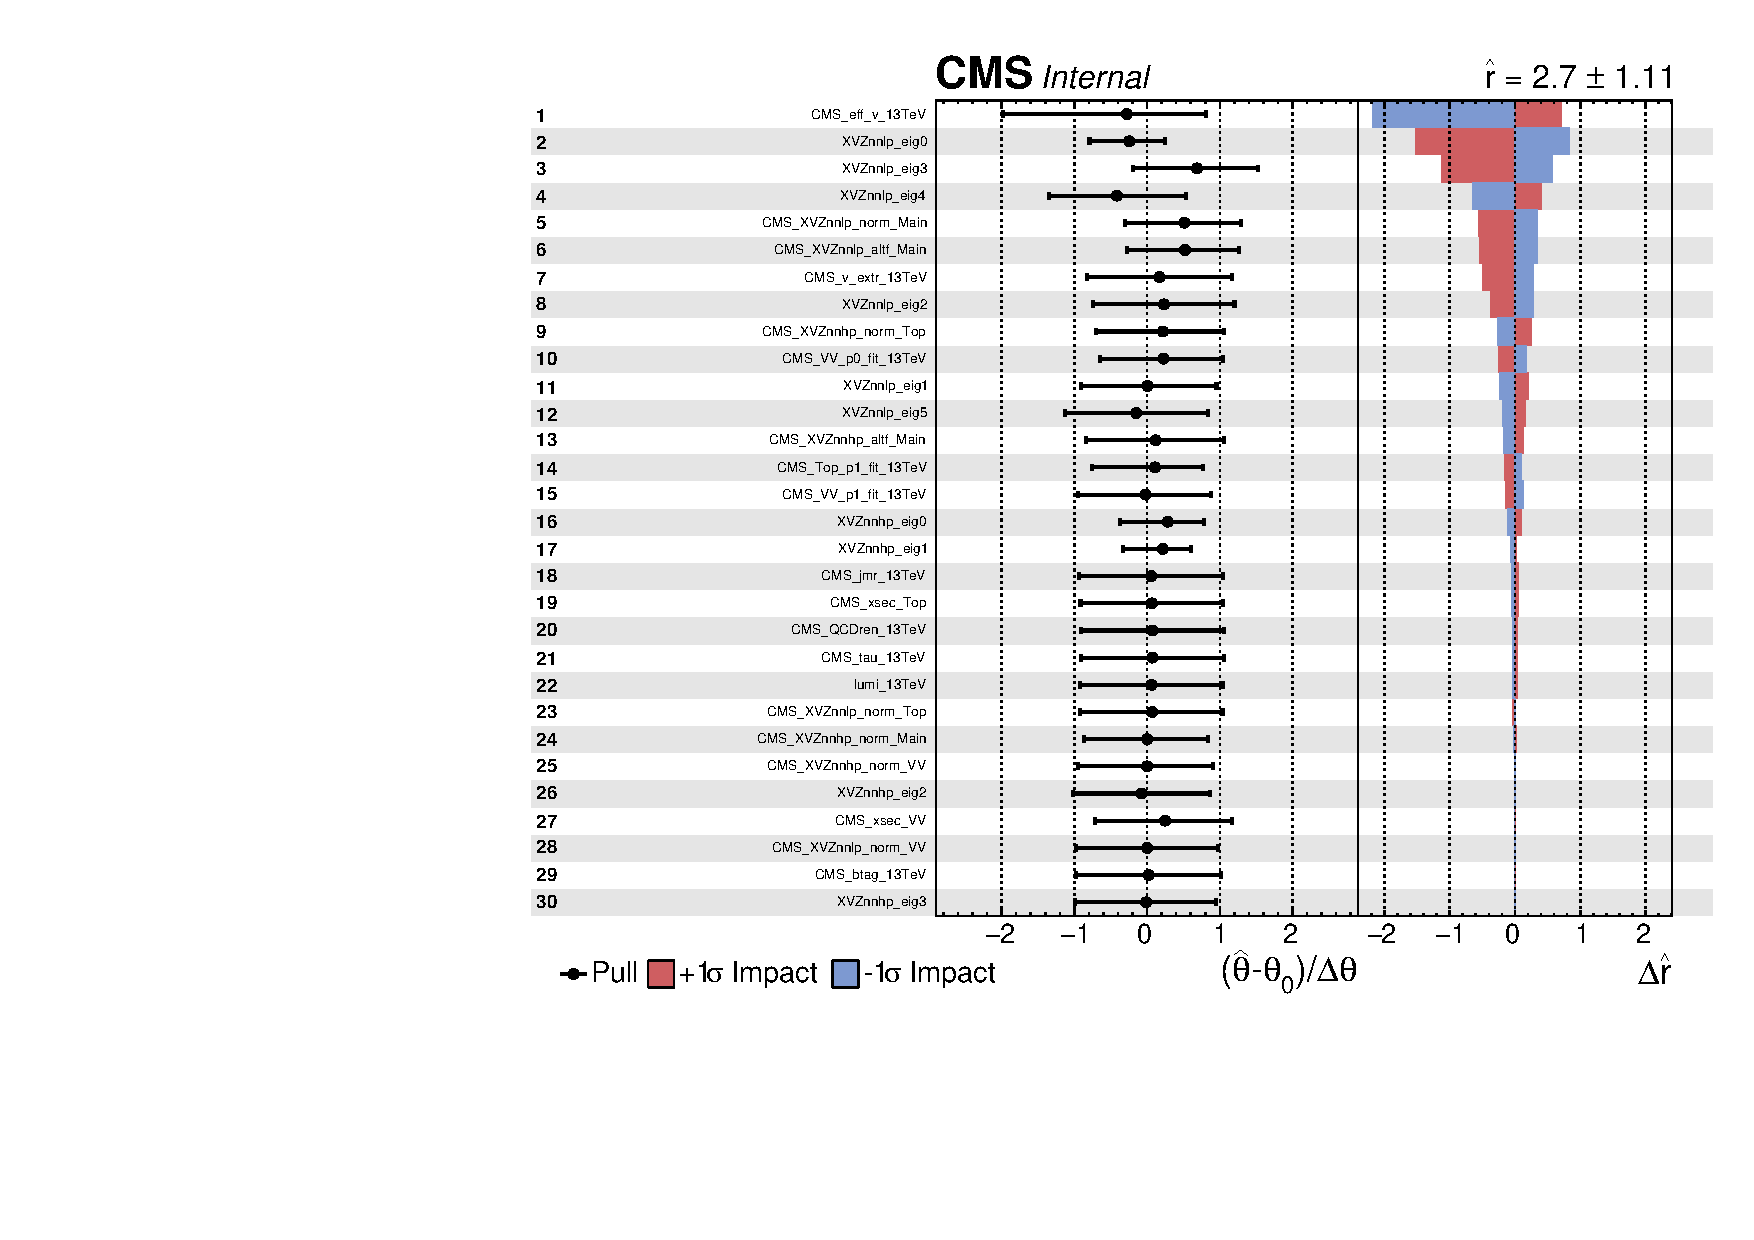
\includegraphics[width=0.75\textwidth]{impacts_VZ_data_1fb/impacts_XZZInv_XVZnn_M2500.pdf}

   \includegraphics[page=2, width=0.75\textwidth]{impacts_VZ_data_1fb/impacts_XZZInv_XVZnn_M2500.pdf}
   \label{fig:impacts}
 \end{center}
\end{figure}


\clearpage

\subsubsection{Results: expected and observed limits}

%Results are obtained from a combined signal and background fit to the unbinned $\mtVZ$ distribution, based on a profile likelihood. Systematic uncertainties are treated as nuisance parameters and are profiled in the statistical interpretation. The background-only hypothesis is tested against the signal in the four categories, and with no evidence of significant deviations from background expectation, the asymptotic modified frequentist method is used to determine the limit at the 95\% confidence level (CL) on the contribution from signal.

The observed upper limits on the resonances cross-sections times branching fraction $\sigma \mathcal{B} (X \rightarrow \V_{\text{had}} \Z_{\text{inv}})$, as well as the expected limits and their relative 68\% and 95\% uncertainty bands, are reported as a function of the resonances masses. The limits are obtained by considering separately a spin-2 bulk graviton and a spin-1 (\Wp) heavy resonances in the narrow-width approximation. For the spin-2 case (fig.~\ref{fig:Limit_XZZInv}), data are compared to theoretical predictions on $\sigma \mathcal{B} (G \rightarrow \Z_{\text{had}} \Z_{\text{inv}})$, obtained by imposing a curvature parameter of the fifth extra-dimension $\tilde{k} = 0.5$ (red curve) and $\tilde{k} = 1.0$ (blue curve). In case of spin-1 hypothesis (fig.\ref{fig:Limit_XWZInv}), HVT model A (red curve) and model B (blue curve) theoretical predictions on $\sigma \mathcal{B} (\Wp \rightarrow \W_{\text{had}} \Z_{\text{inv}})$ are reported.

\noindent Given the fact that the background prediction is performed in a transverse mass range $950~<$~\mtVZ~$<4750$~\GeV of the resonance, and given that the higher the nominal mass of the resonance, the more the Crystal Ball functions, parametrizing the \mtVZ distributions of both spin-1 and spin-2 signals, tend to have low-mass tails (sec.~\ref{ssec:signal_parametrization}), a safe conservative criterion is to set limits in the resonance mass range 1 \TeV -- 4 \TeV.

\noindent No significant excess is observed in data with respect to the background-only hypothesis, neither in the low-purity, nor in the high-purity category. As it can be inferred by fig.~\ref{fig:Limit_XZZInv}-\ref{fig:Limit_XWZInv}, low-purity category has a larger sensitivity to both spin-1 and spin-2 signals in the high mass region, whilst high-purity category is more sensitive at low masses. This reflects the different signal efficiencies of the two categories, as discussed in sec.~\ref{sec:selections} (fig.~\ref{fig:eff_n}). By combining the two categories, the best exclusion limits can be determined. Upper limits on the $\sigma \mathcal{B} (X \rightarrow \V_{\text{had}} \Z_{\text{inv}})$ of heavy spin-2 and spin-1 narrow resonances are set in the range $0.5$ -- $40$ \fb and in the range $0.9$ -- $63$ \fb respectively. A spin-2 bulk-graviton, once assumed a curvature parameter $\tilde{k} = 1.0$, is excluded up to 1.14 \TeV. A spin-1 \Wp, predicted by the model A scenario ($g_V=1$), is excluded up to a mass of 3.11 \TeV. A spin-1 \Wp, predicted by the model B scenario ($g_V=3$), is excluded up to a mass of 3.41 \TeV. 


\begin{figure}[!htb]
  \begin{center}
     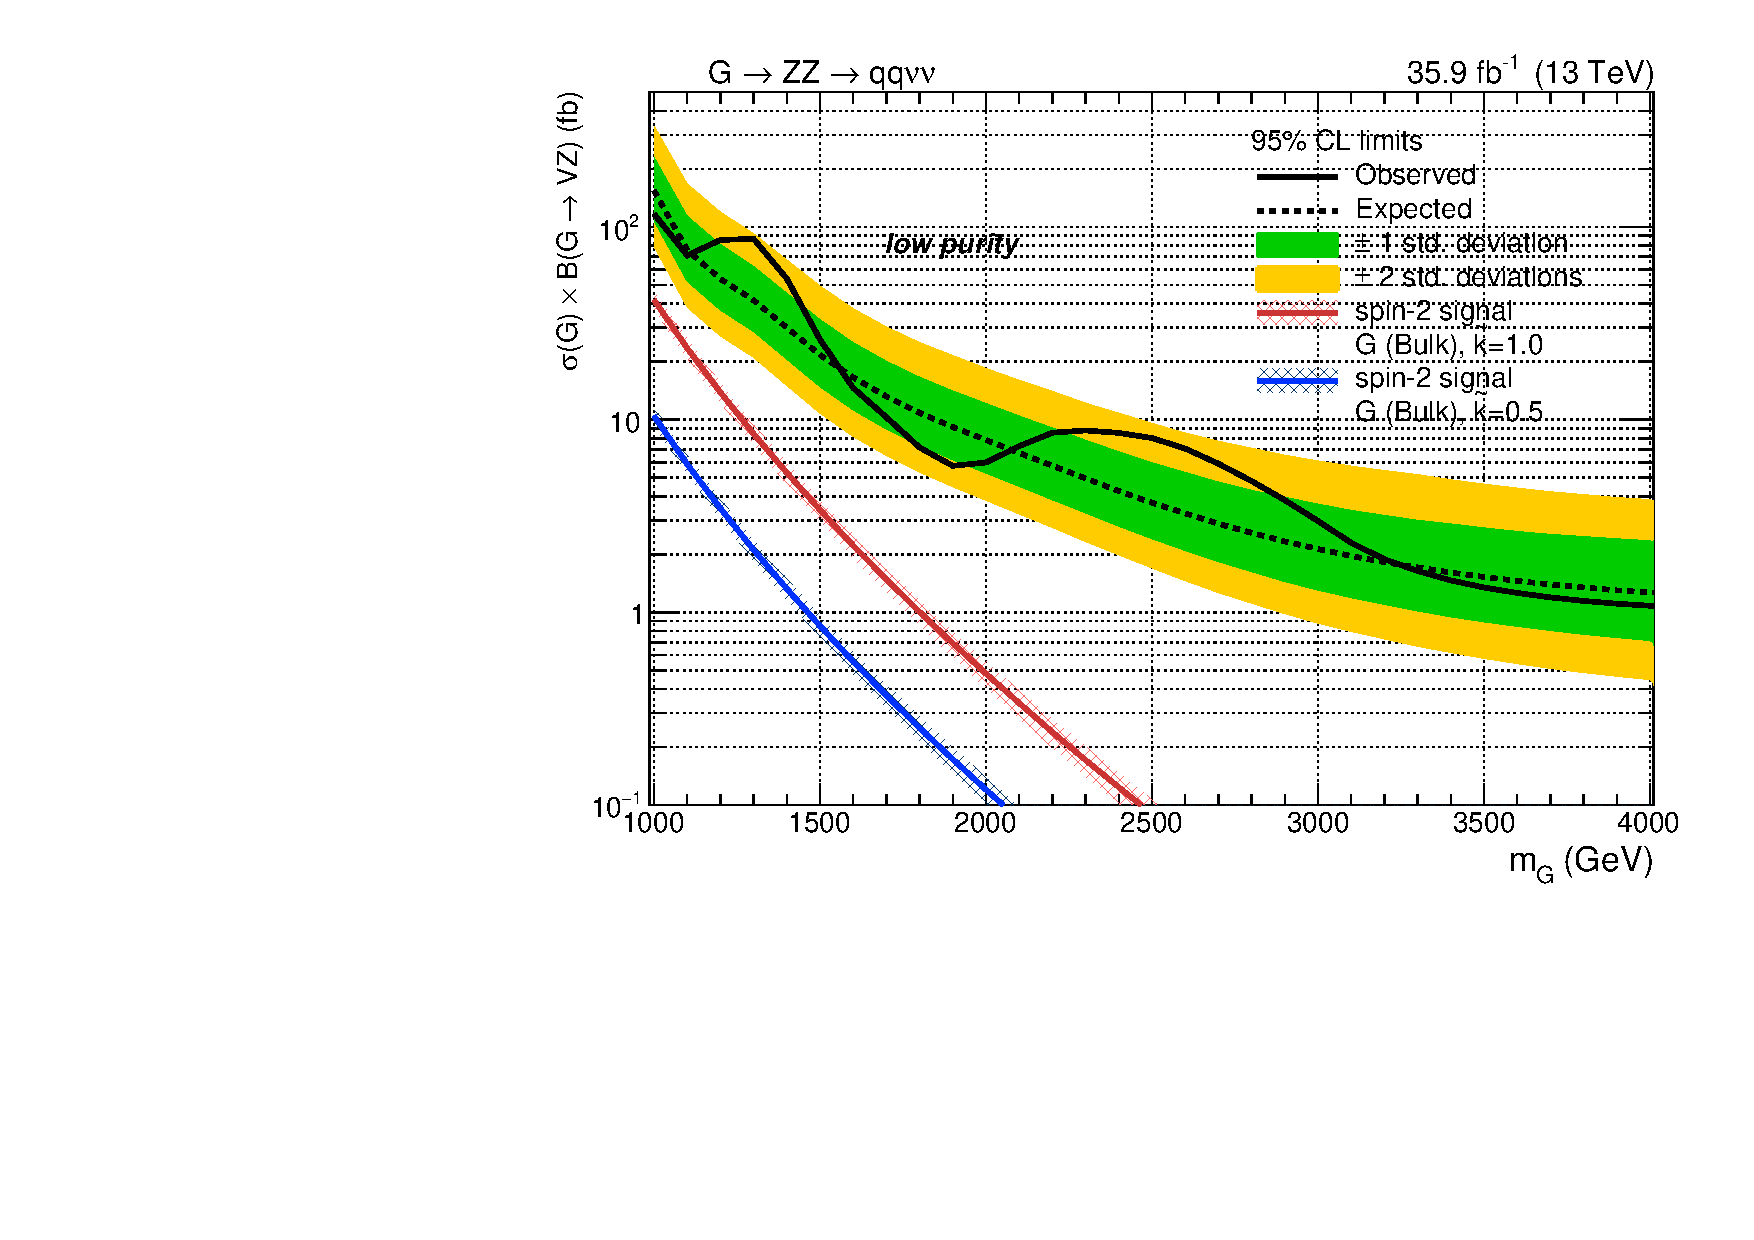
\includegraphics[width=.495\textwidth]{plotsAlpha_tesi/Limits/Exclusion_XZZInv_XVZnnlp1p0_asymptotic.pdf}%
     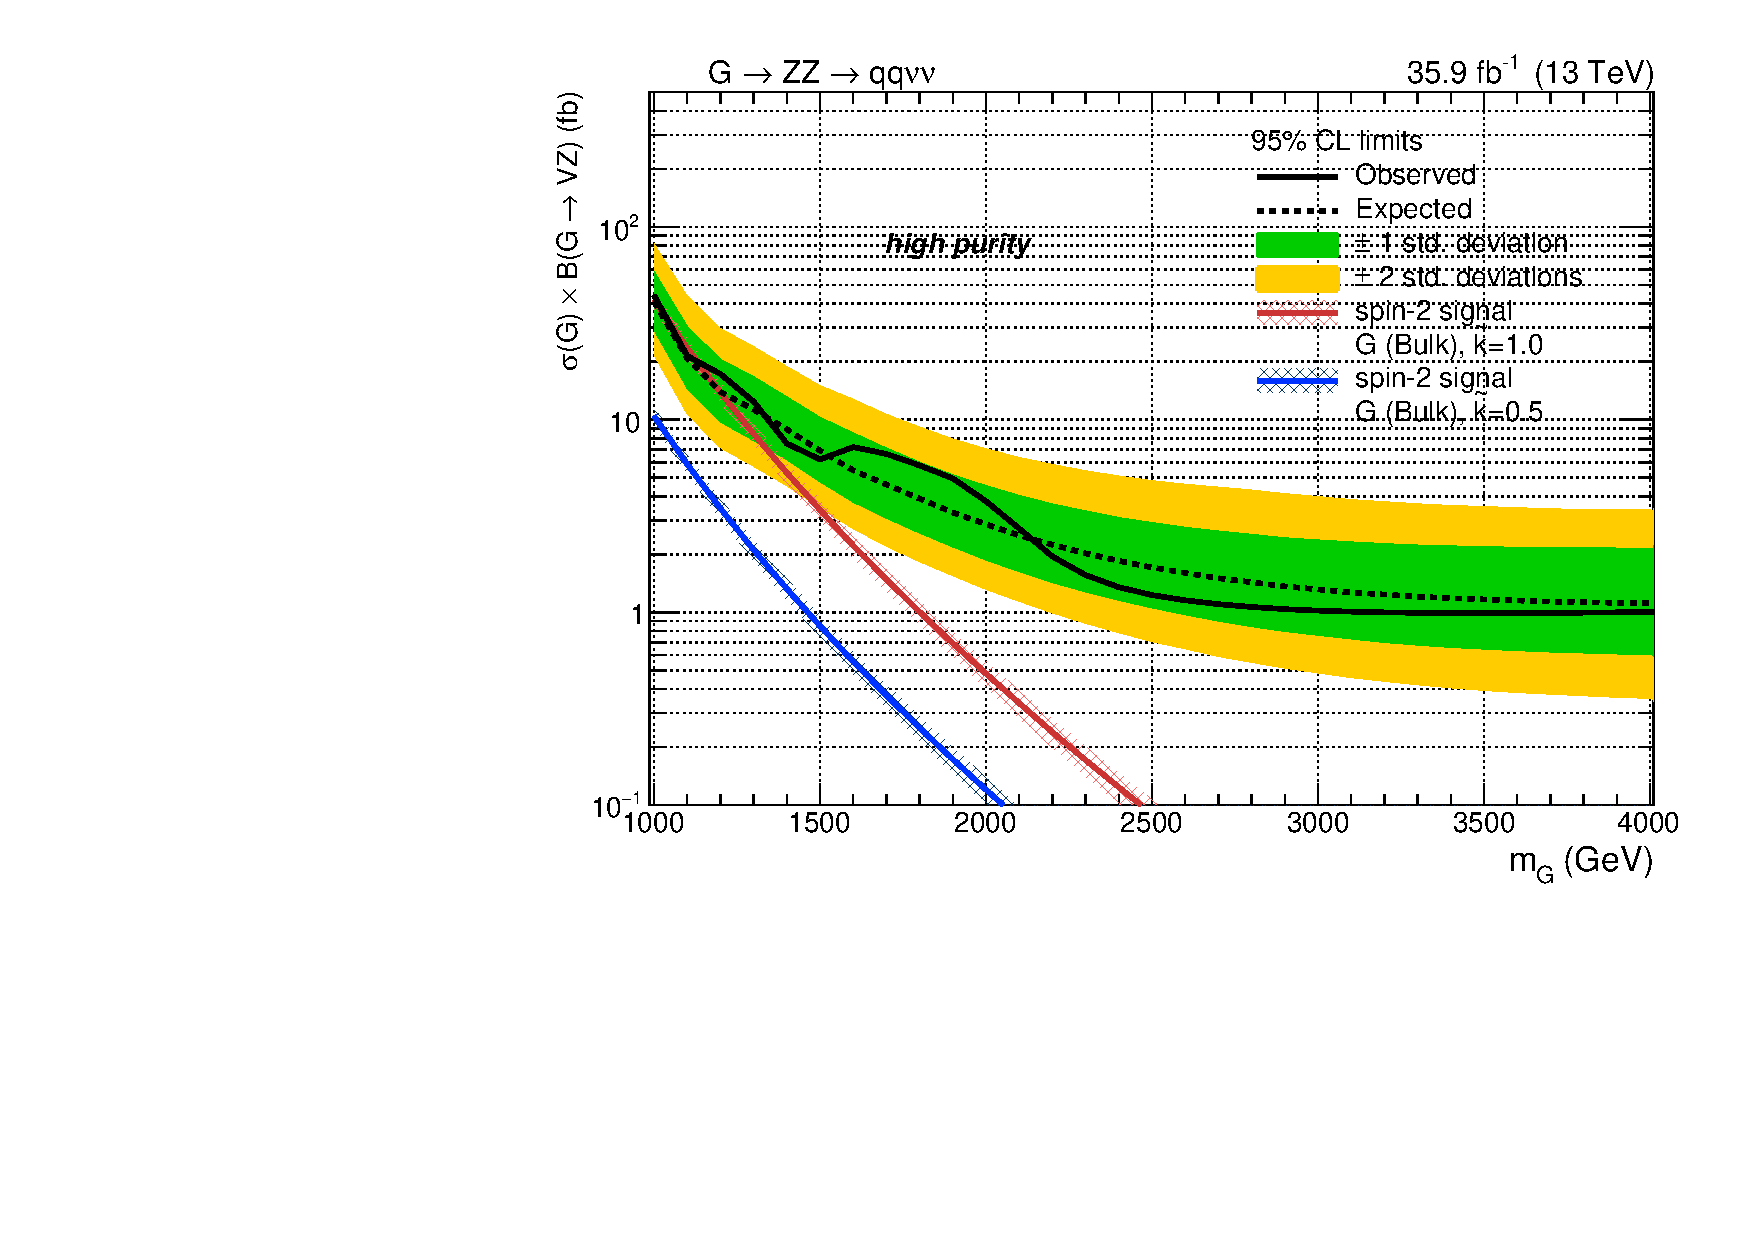
\includegraphics[width=.495\textwidth]{plotsAlpha_tesi/Limits/Exclusion_XZZInv_XVZnnhp1p0_asymptotic.pdf}

     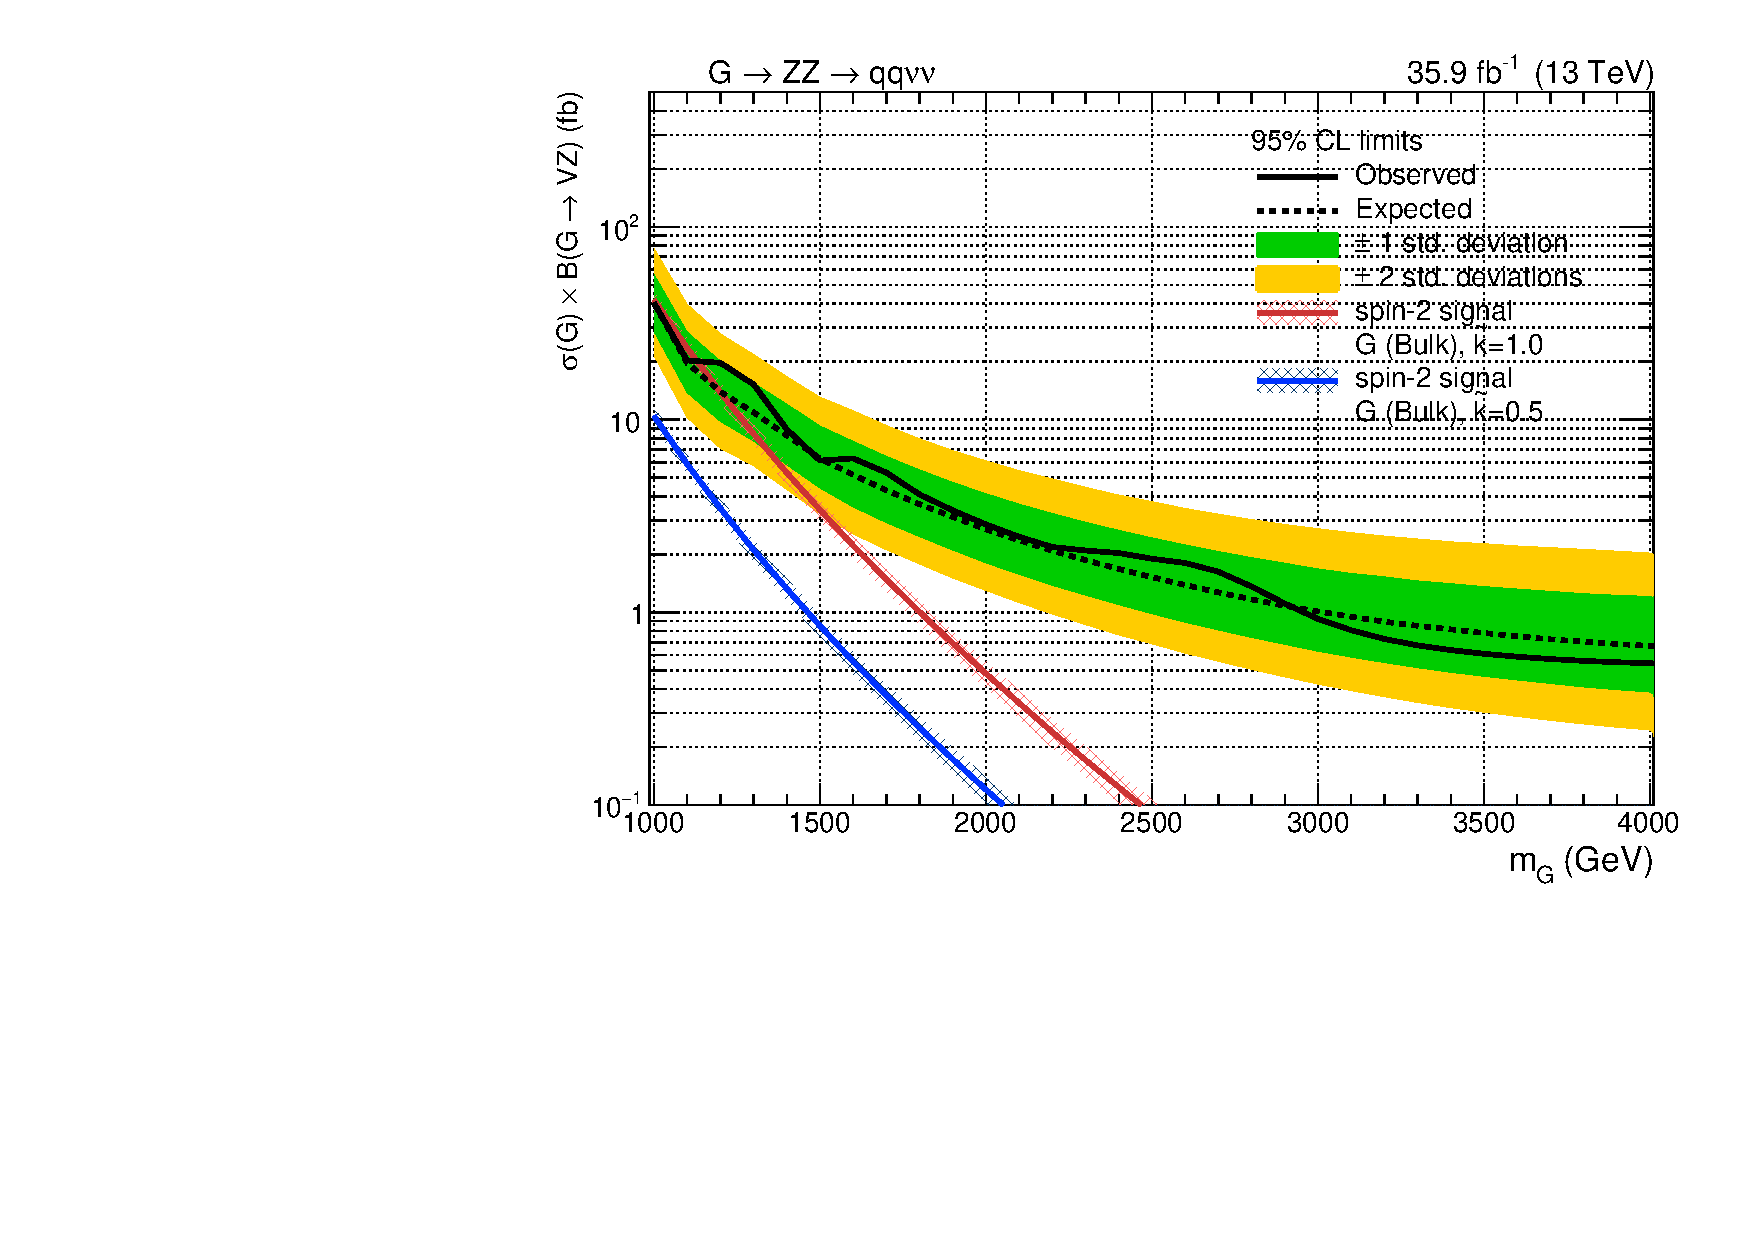
\includegraphics[width=.495\textwidth]{plotsAlpha_tesi/Limits/Exclusion_XZZInv_XVZnn1p0_asymptotic.pdf}
  \end{center}
  \caption{Top: observed and expected (with $\pm1(2)\sigma$ band) 95\% C.L. upper limit on $\sigma \mathcal{B} (\G \rightarrow \Z_{\text{had}} \Z_{\text{inv}})$ for a spin-2 (bulk graviton) signal, for low-purity (left) and high-purity (right) categories, including all statistical and systematics uncertainties. Background predictions are extracted with the $\alpha$ method. Bottom: observed and expected (with $\pm1(2)\sigma$ band) 95\% C.L. upper limit on $\sigma \mathcal{B} (\G \rightarrow \Z_{\text{had}} \Z_{\text{inv}})$ for a spin-2 (bulk graviton) signal, combining the two purity categories.}
  \label{fig:Limit_XZZInv}
\end{figure}

\begin{figure}[!htb]
  \begin{center}
     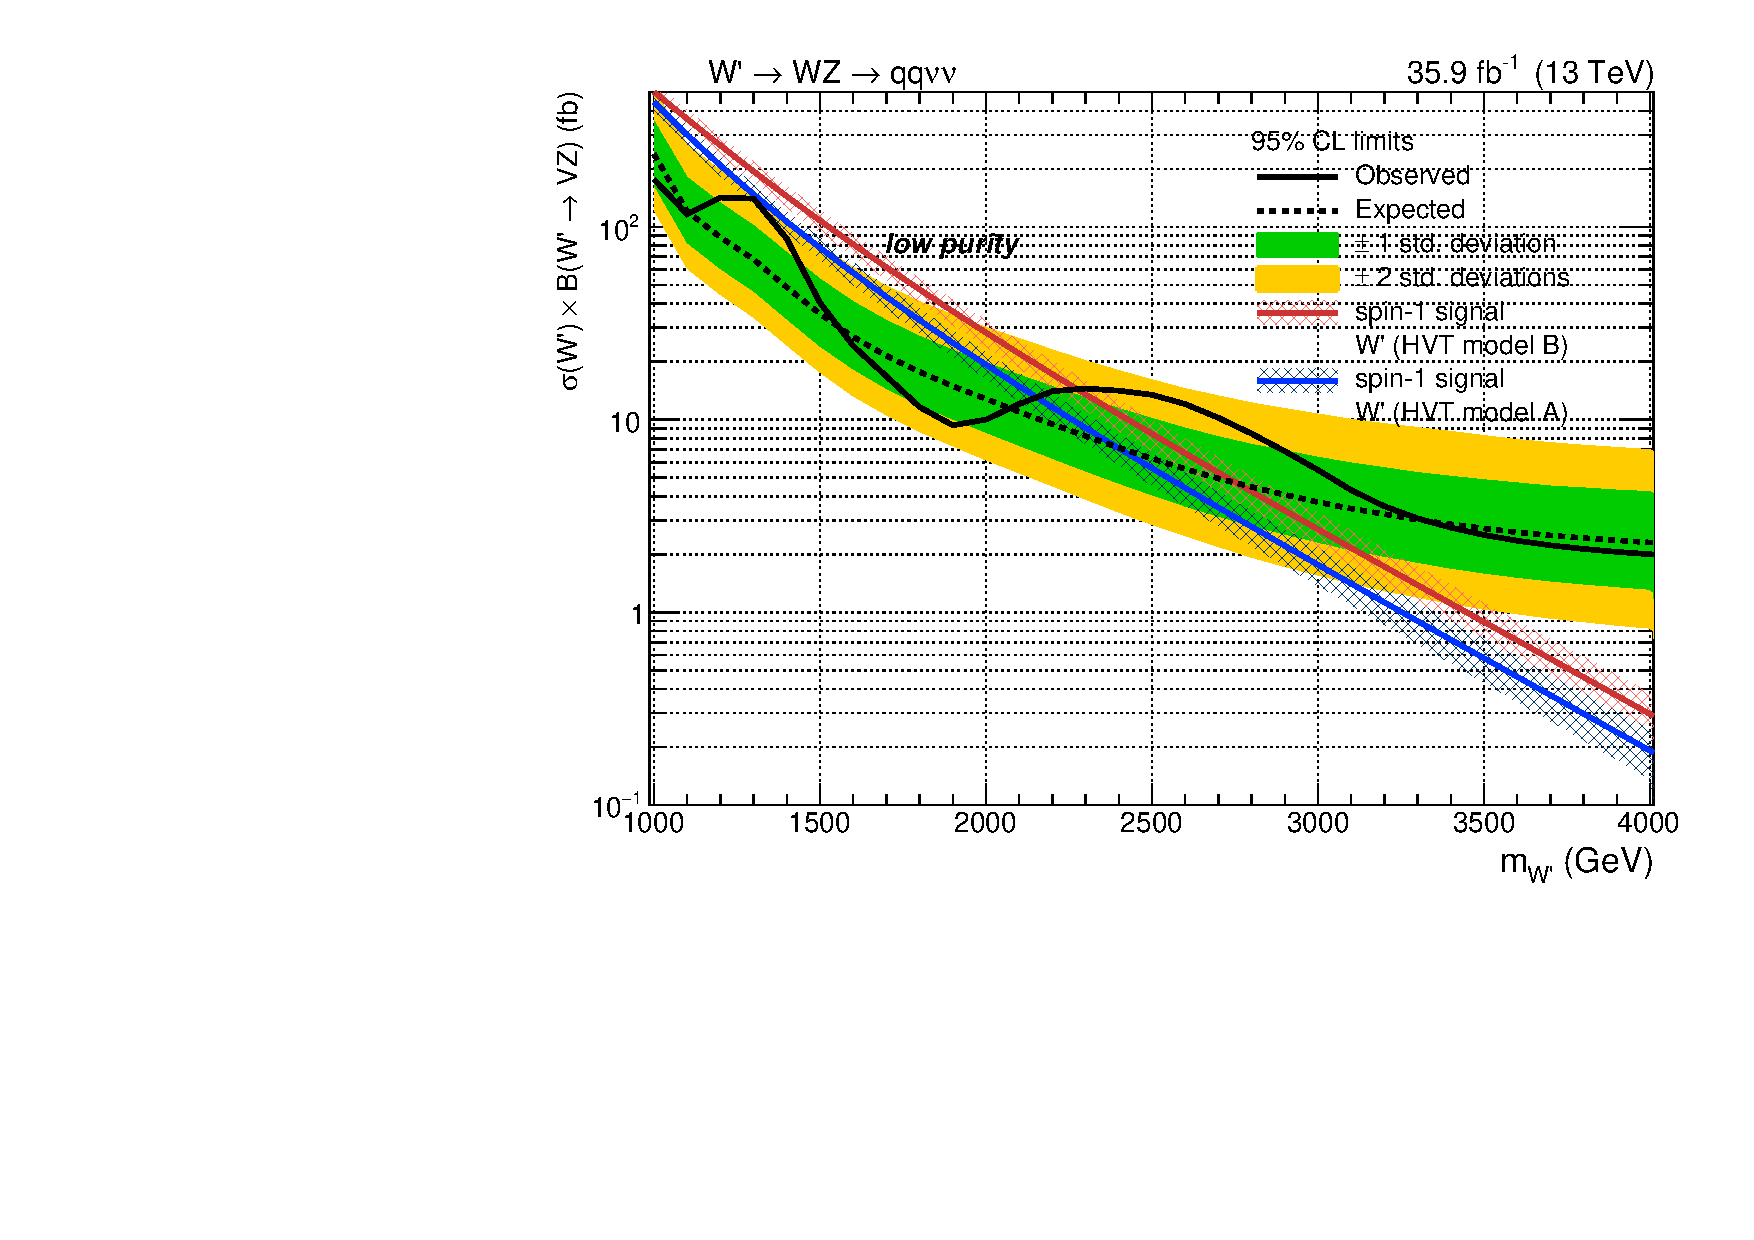
\includegraphics[width=.495\textwidth]{plotsAlpha_tesi/Limits/Exclusion_XWZInv_XVZnnlp_asymptotic.pdf}%
     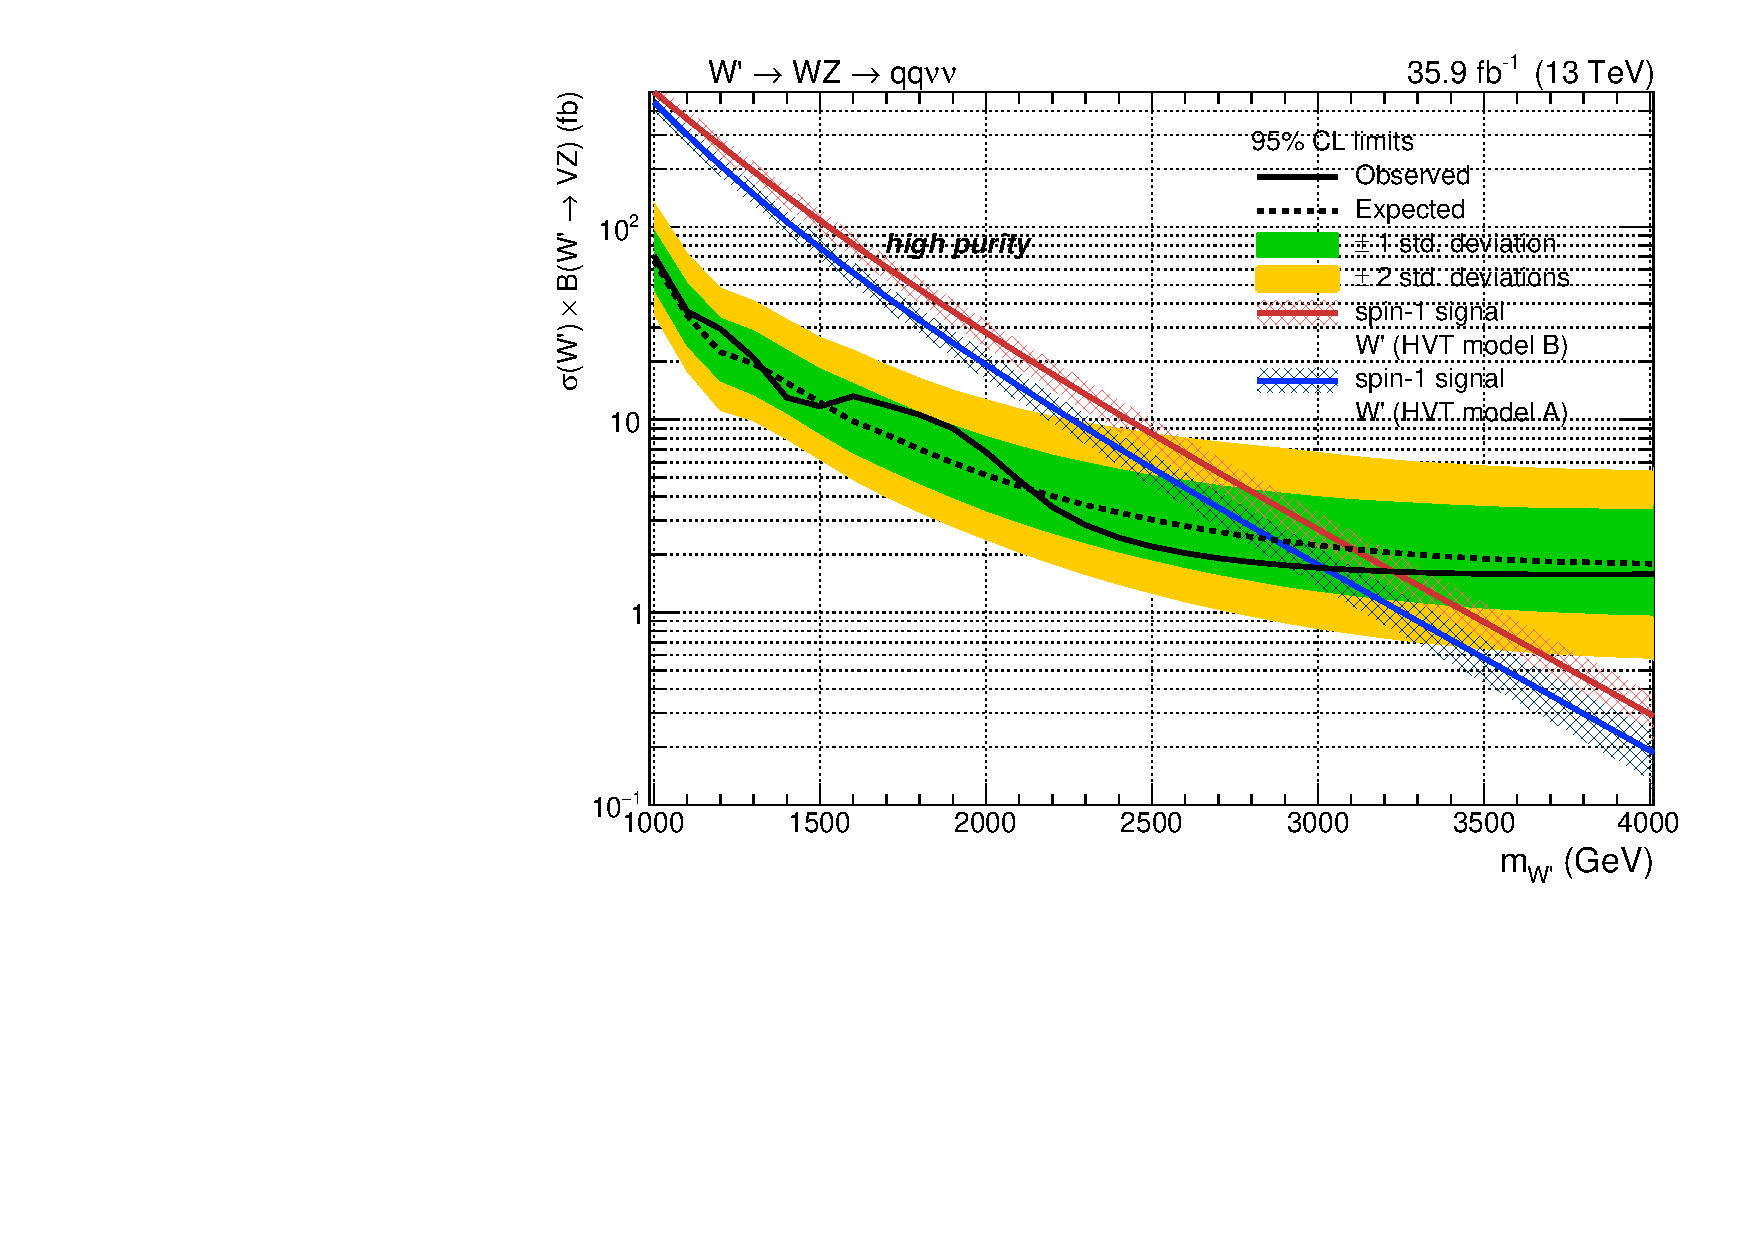
\includegraphics[width=.495\textwidth]{plotsAlpha_tesi/Limits/Exclusion_XWZInv_XVZnnhp_asymptotic.pdf}

     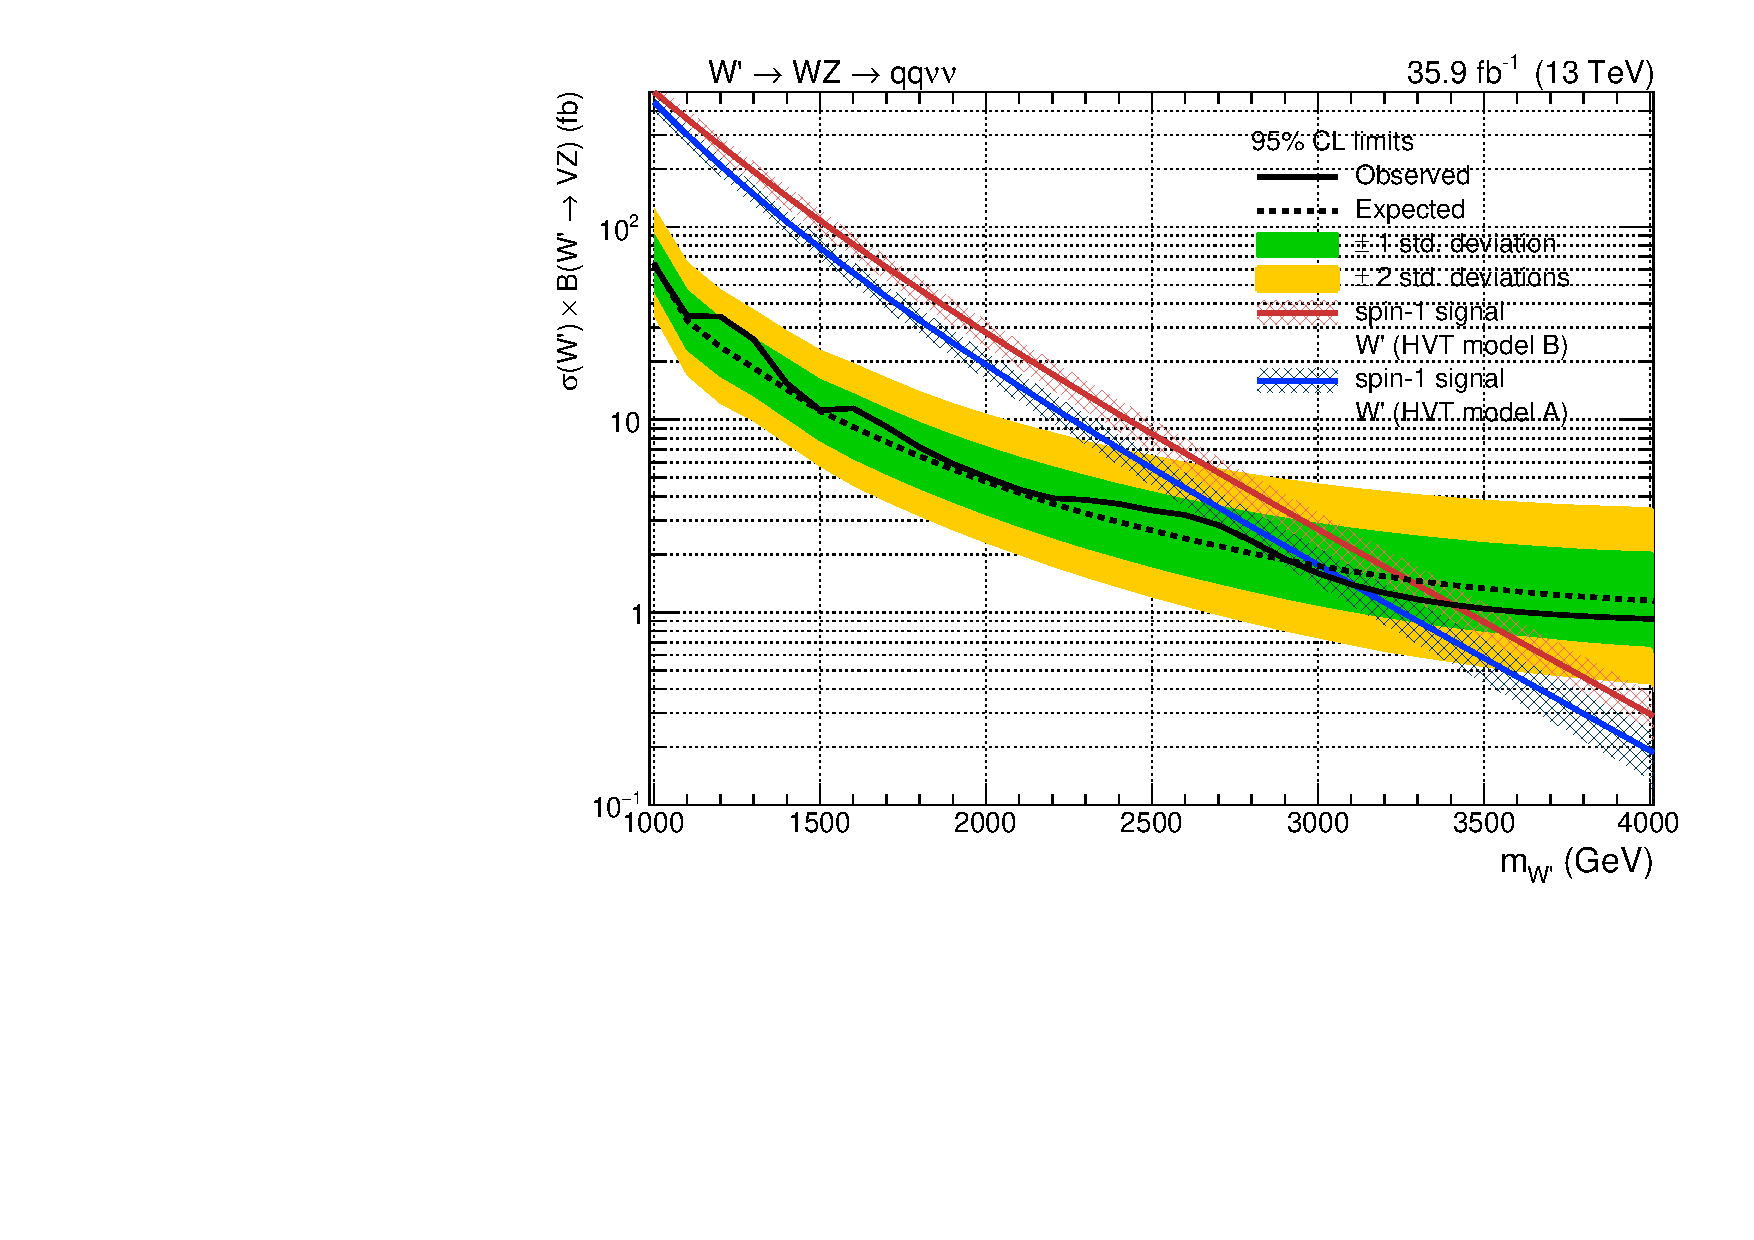
\includegraphics[width=.495\textwidth]{plotsAlpha_tesi/Limits/Exclusion_XWZInv_XVZnn_asymptotic.pdf}
  \end{center}
  \caption{Top: observed and expected (with $\pm1(2)\sigma$ band) 95\% C.L. upper limit on $\sigma \mathcal{B} (\Wp \rightarrow \W_{\text{had}} \Z_{\text{inv}})$ for a spin-1 (HVT) signal, for low-purity (left) and high-purity (right) categories, including all statistical and systematics uncertainties. Background predictions are extracted with the $\alpha$ method. Bottom: observed and expected (with $\pm1(2)\sigma$ band) 95\% C.L. upper limit on $\sigma \mathcal{B} (\Wp \rightarrow \W_{\text{had}} \Z_{\text{inv}})$ for a spin-1 (HVT) signal, combining the two purity categories.}
  \label{fig:Limit_XWZInv}
\end{figure}

\subsubsection{Results: local p-value scan}
Scans of the local significances (left plots) and of the local p-values (right plots), as a function of the resonance mass, are presented in fig.~\ref{fig:Signif_XZZInv} (spin-2 signal) and in fig.~\ref{fig:Signif_XWZInv} (spin-1 signal). No significant deviation is observed with regards to the background-only hypothesis. The maximum deviation is observed in the low-purity category, around 1.3 and 2.5 \TeV, and it amounts to $\sim 2 \sigma$. For the combination of the categories, data are compatible with the background-only hypothesis within $1 \sigma$ in the whole mass spectrum.

\begin{figure}[!htb]
  \begin{center}
     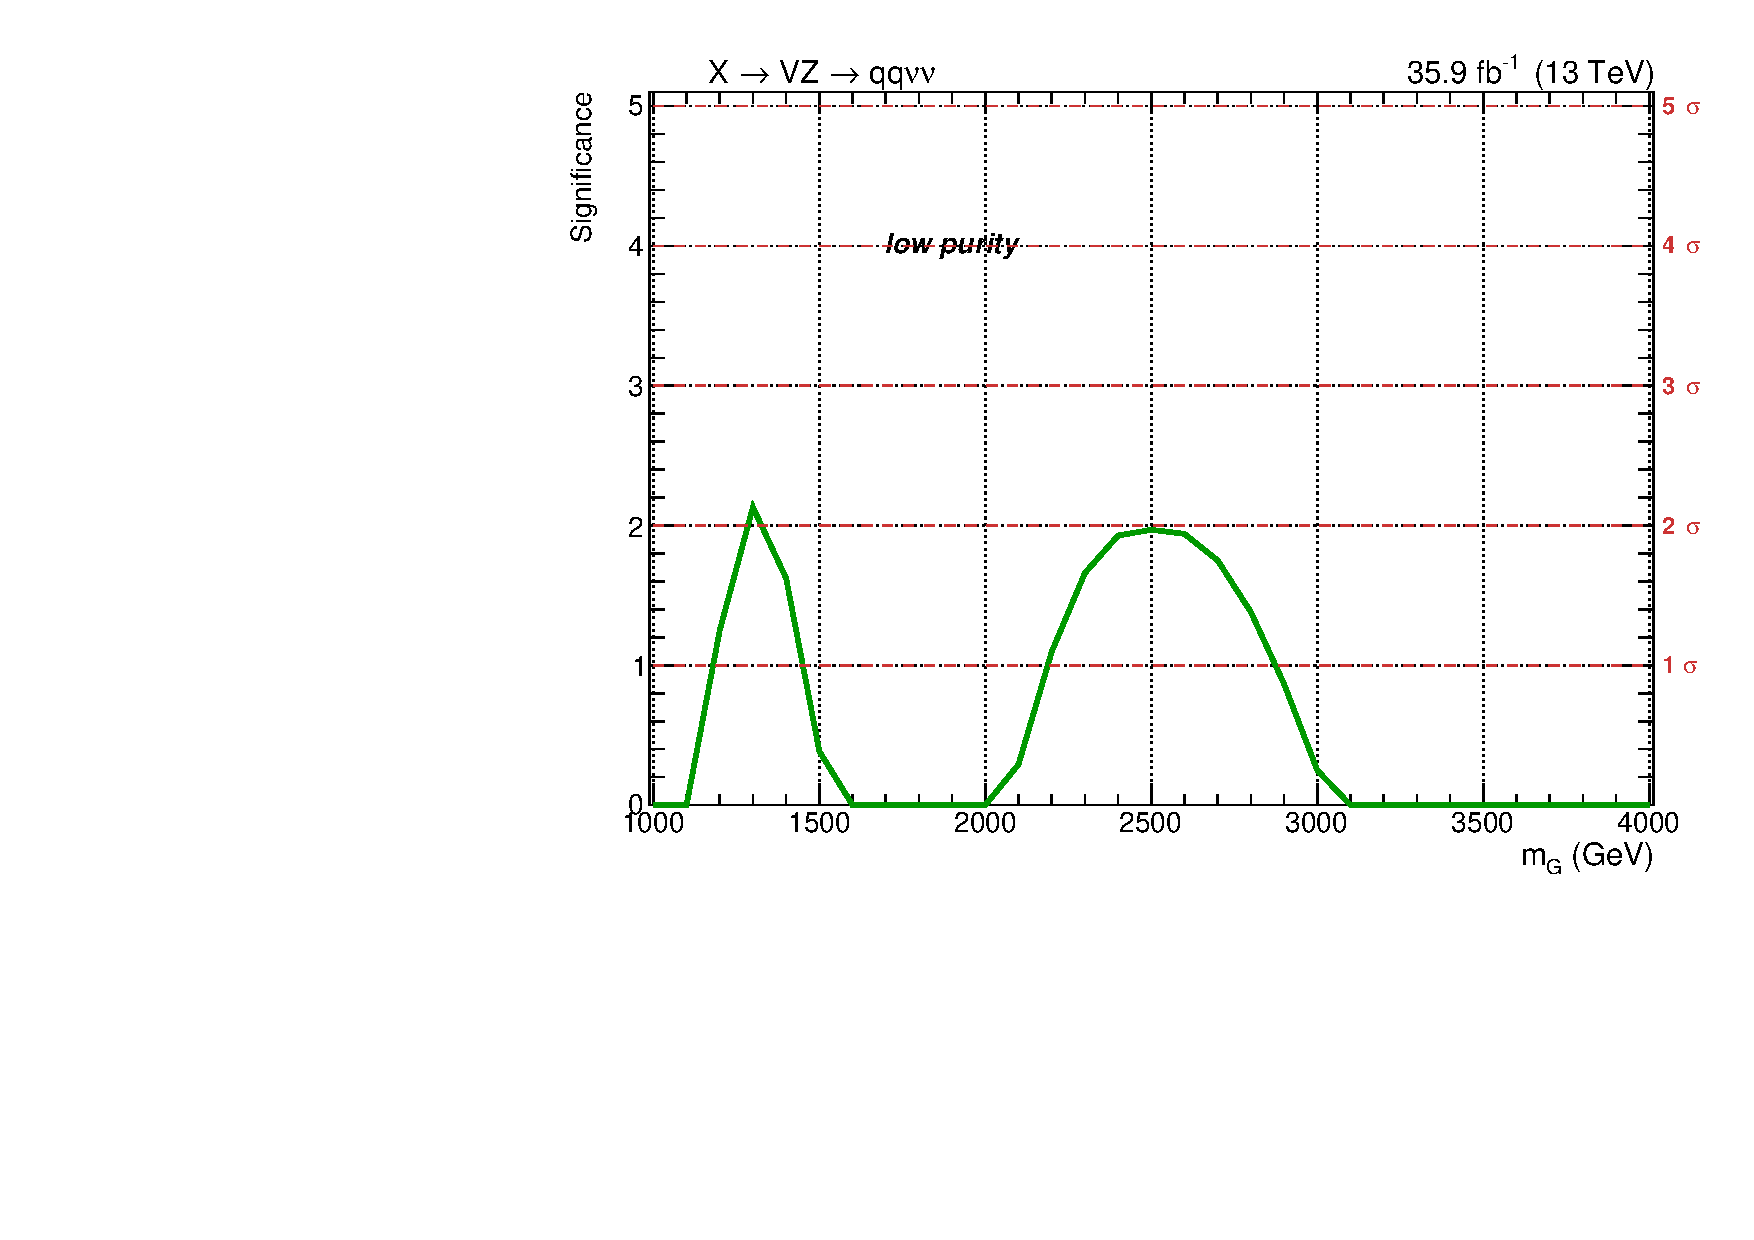
\includegraphics[width=.495\textwidth]{plotsAlpha_tesi/Limits/Significance_XZZInv_XVZnnlp.pdf}%
     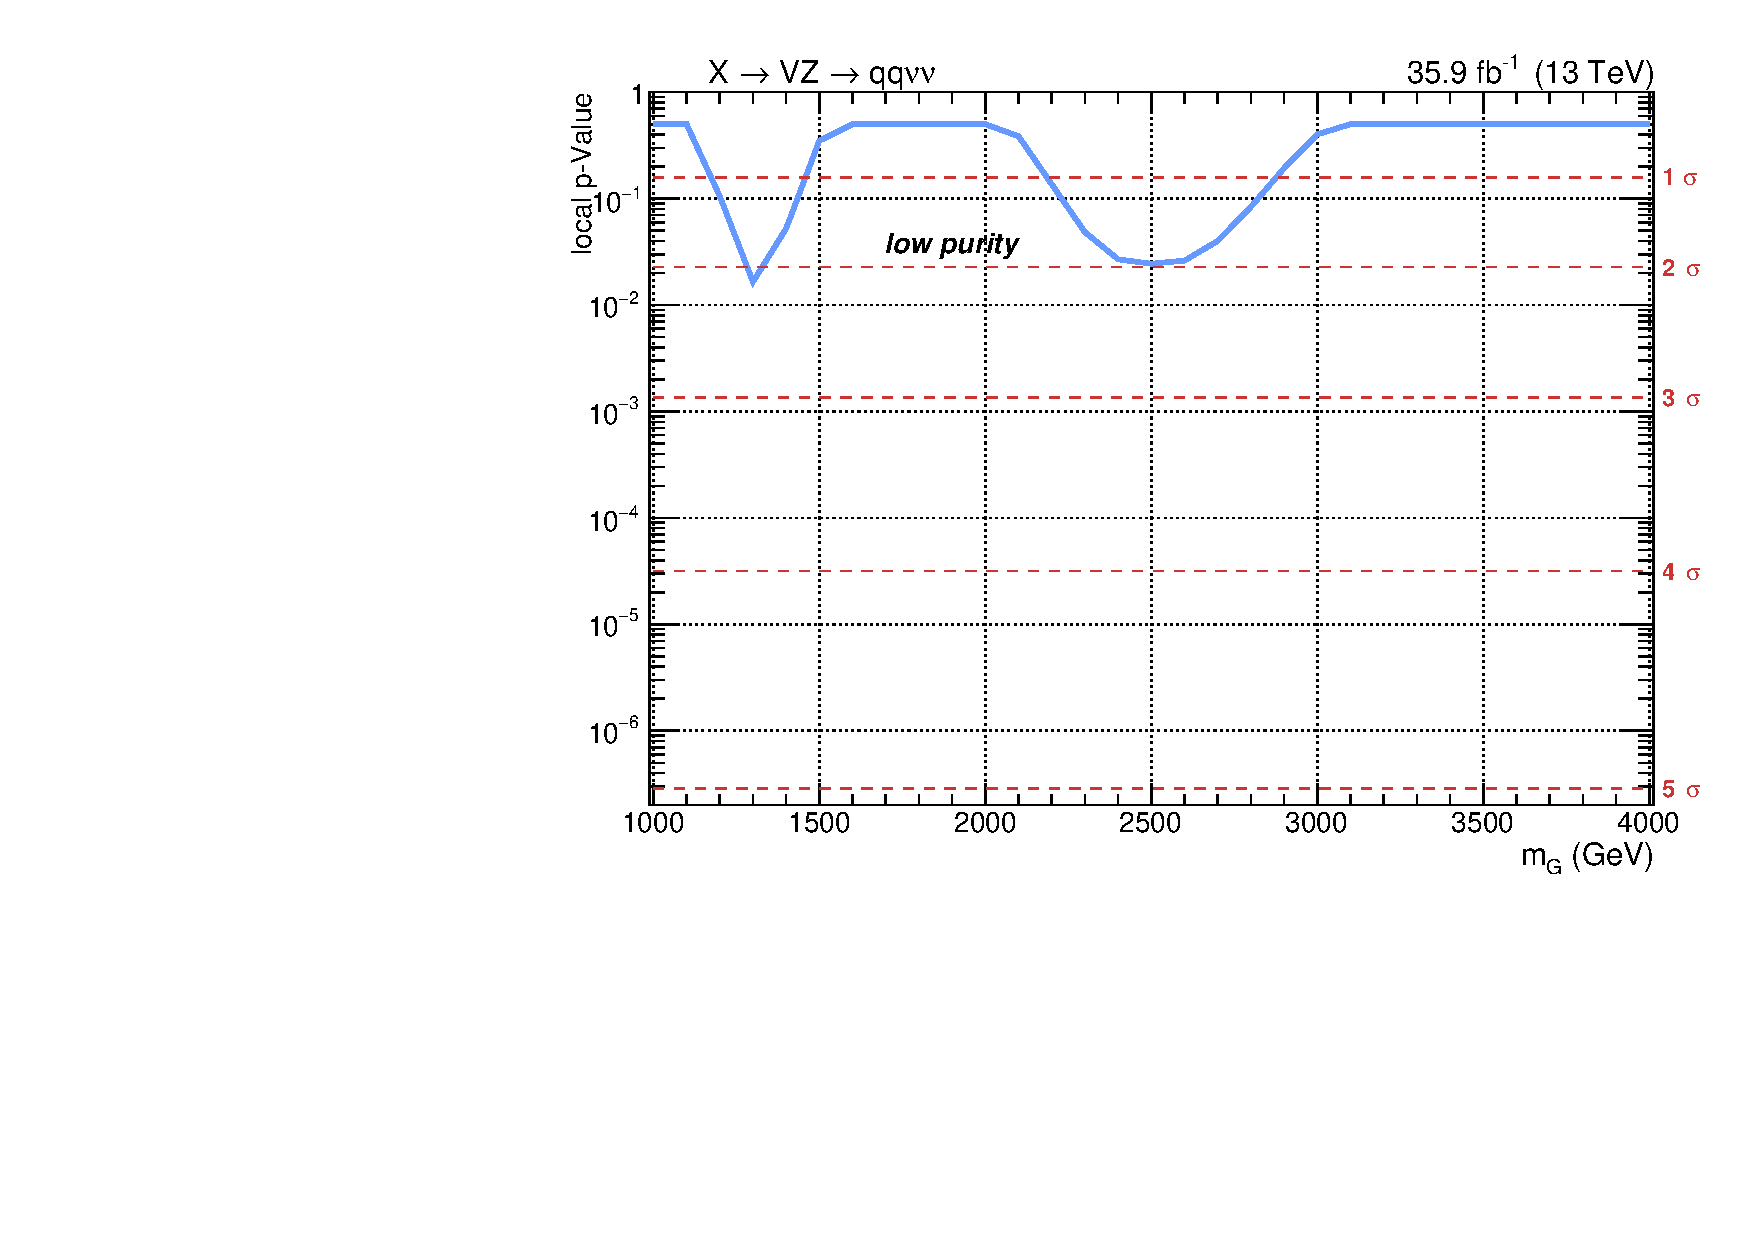
\includegraphics[width=.495\textwidth]{plotsAlpha_tesi/Limits/pValue_XZZInv_XVZnnlp.pdf}

     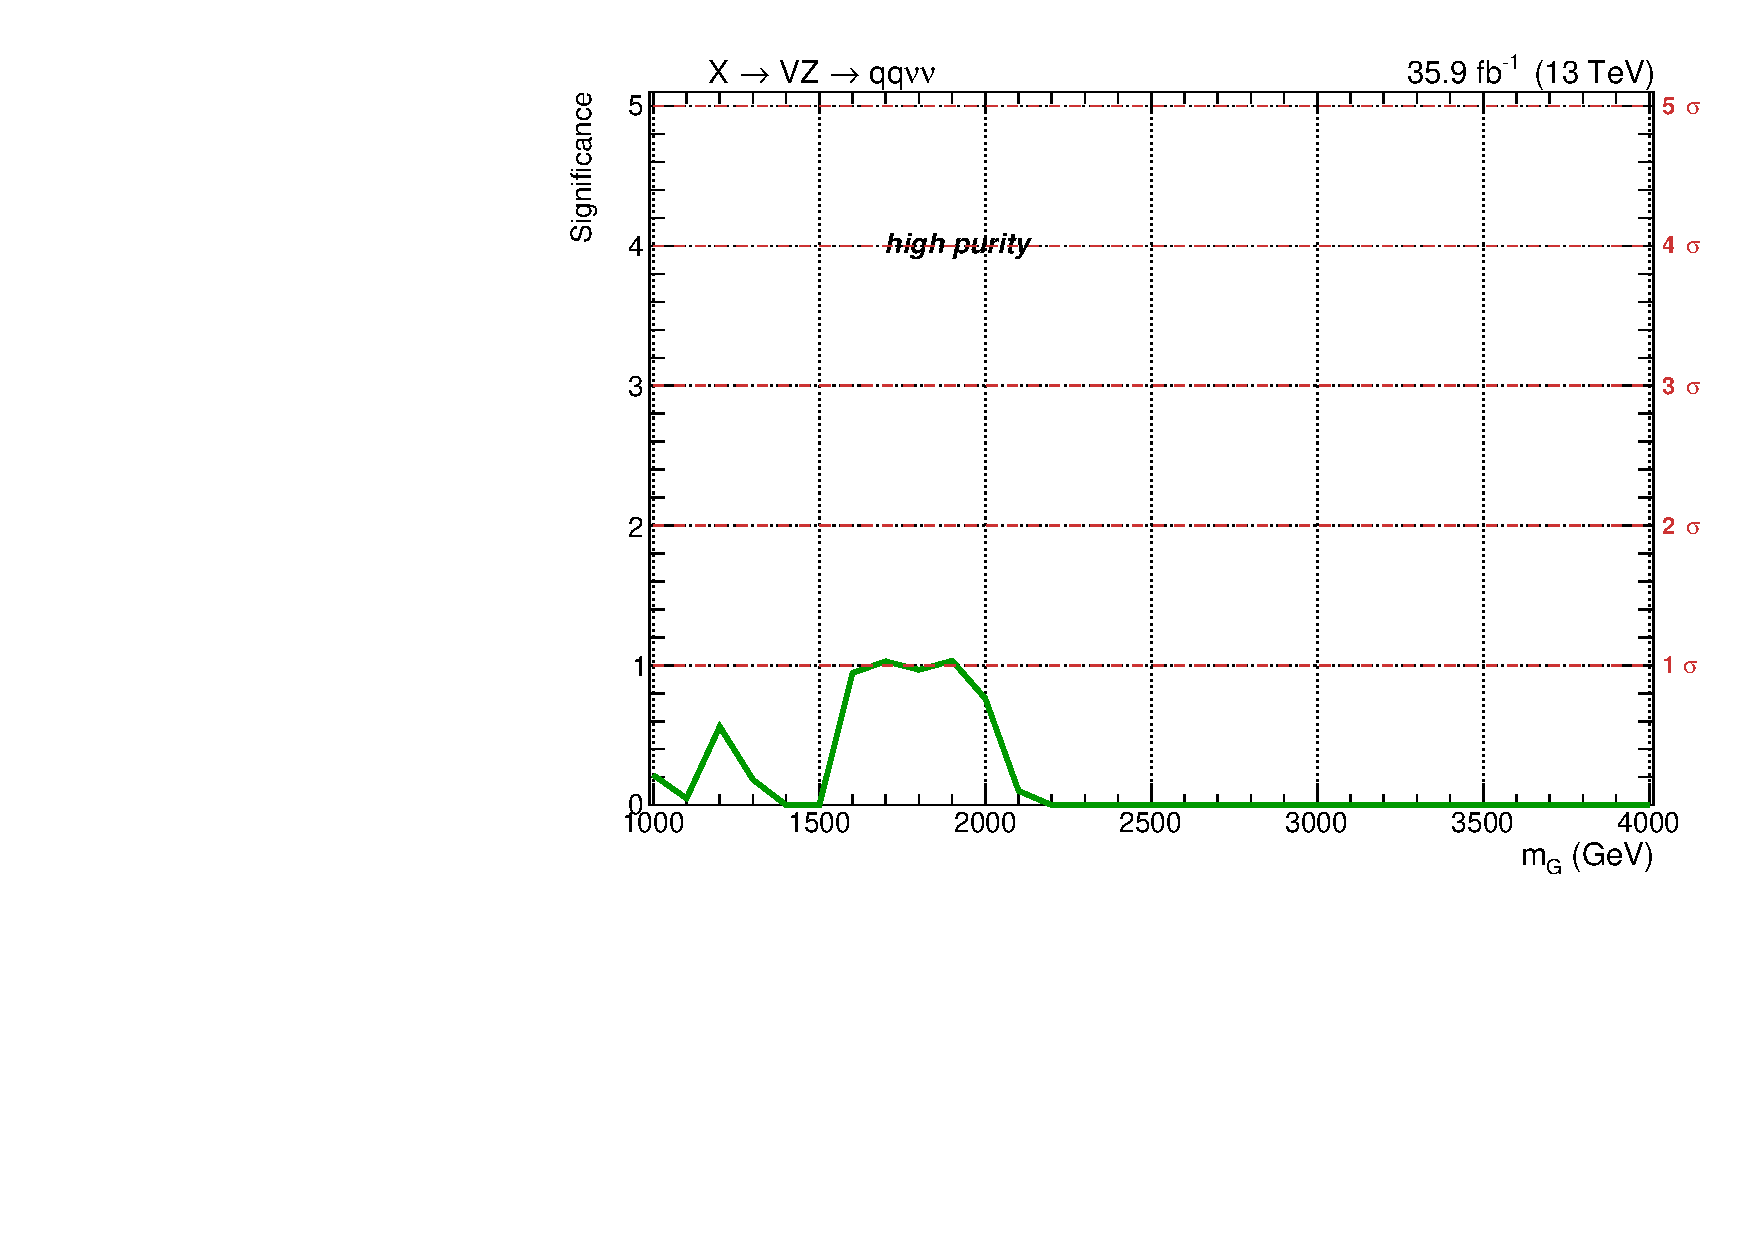
\includegraphics[width=.495\textwidth]{plotsAlpha_tesi/Limits/Significance_XZZInv_XVZnnhp.pdf}%
     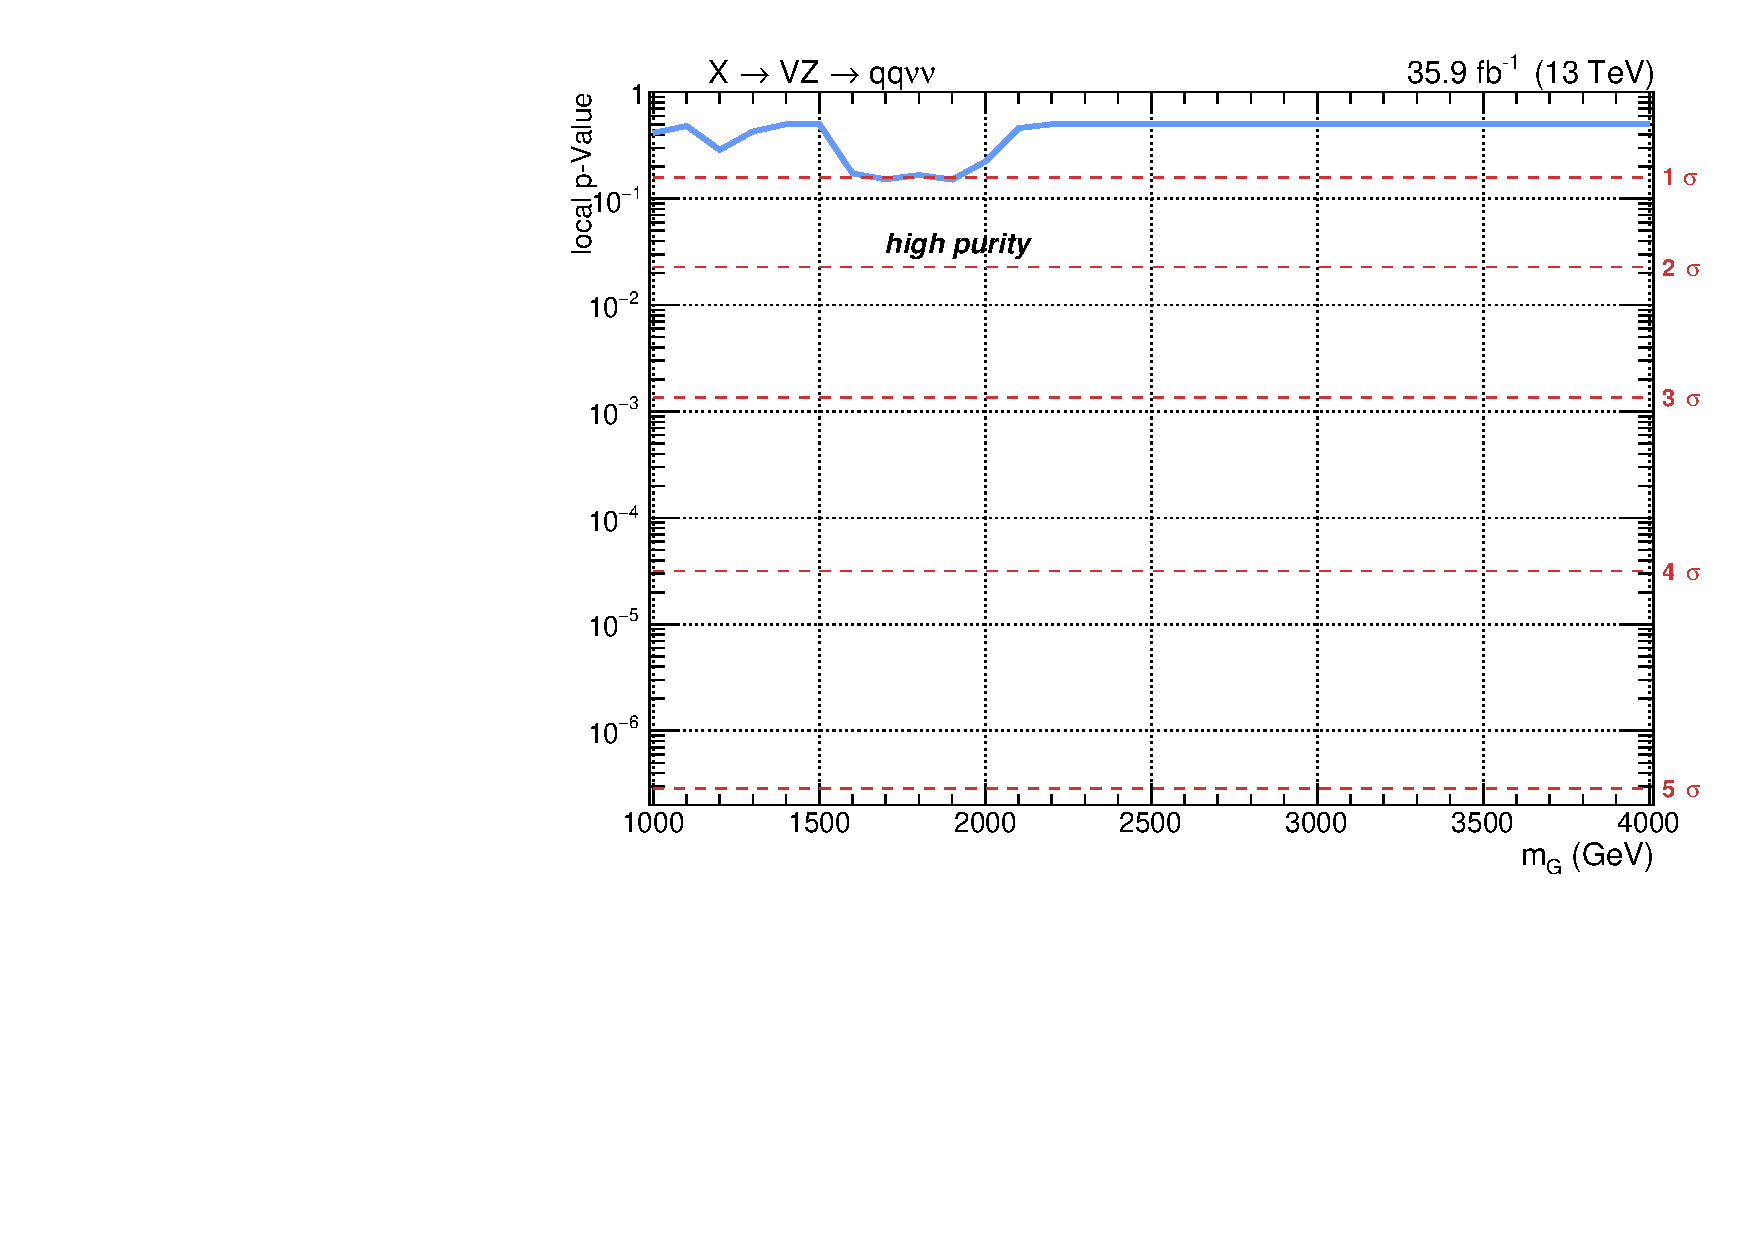
\includegraphics[width=.495\textwidth]{plotsAlpha_tesi/Limits/pValue_XZZInv_XVZnnhp.pdf}

     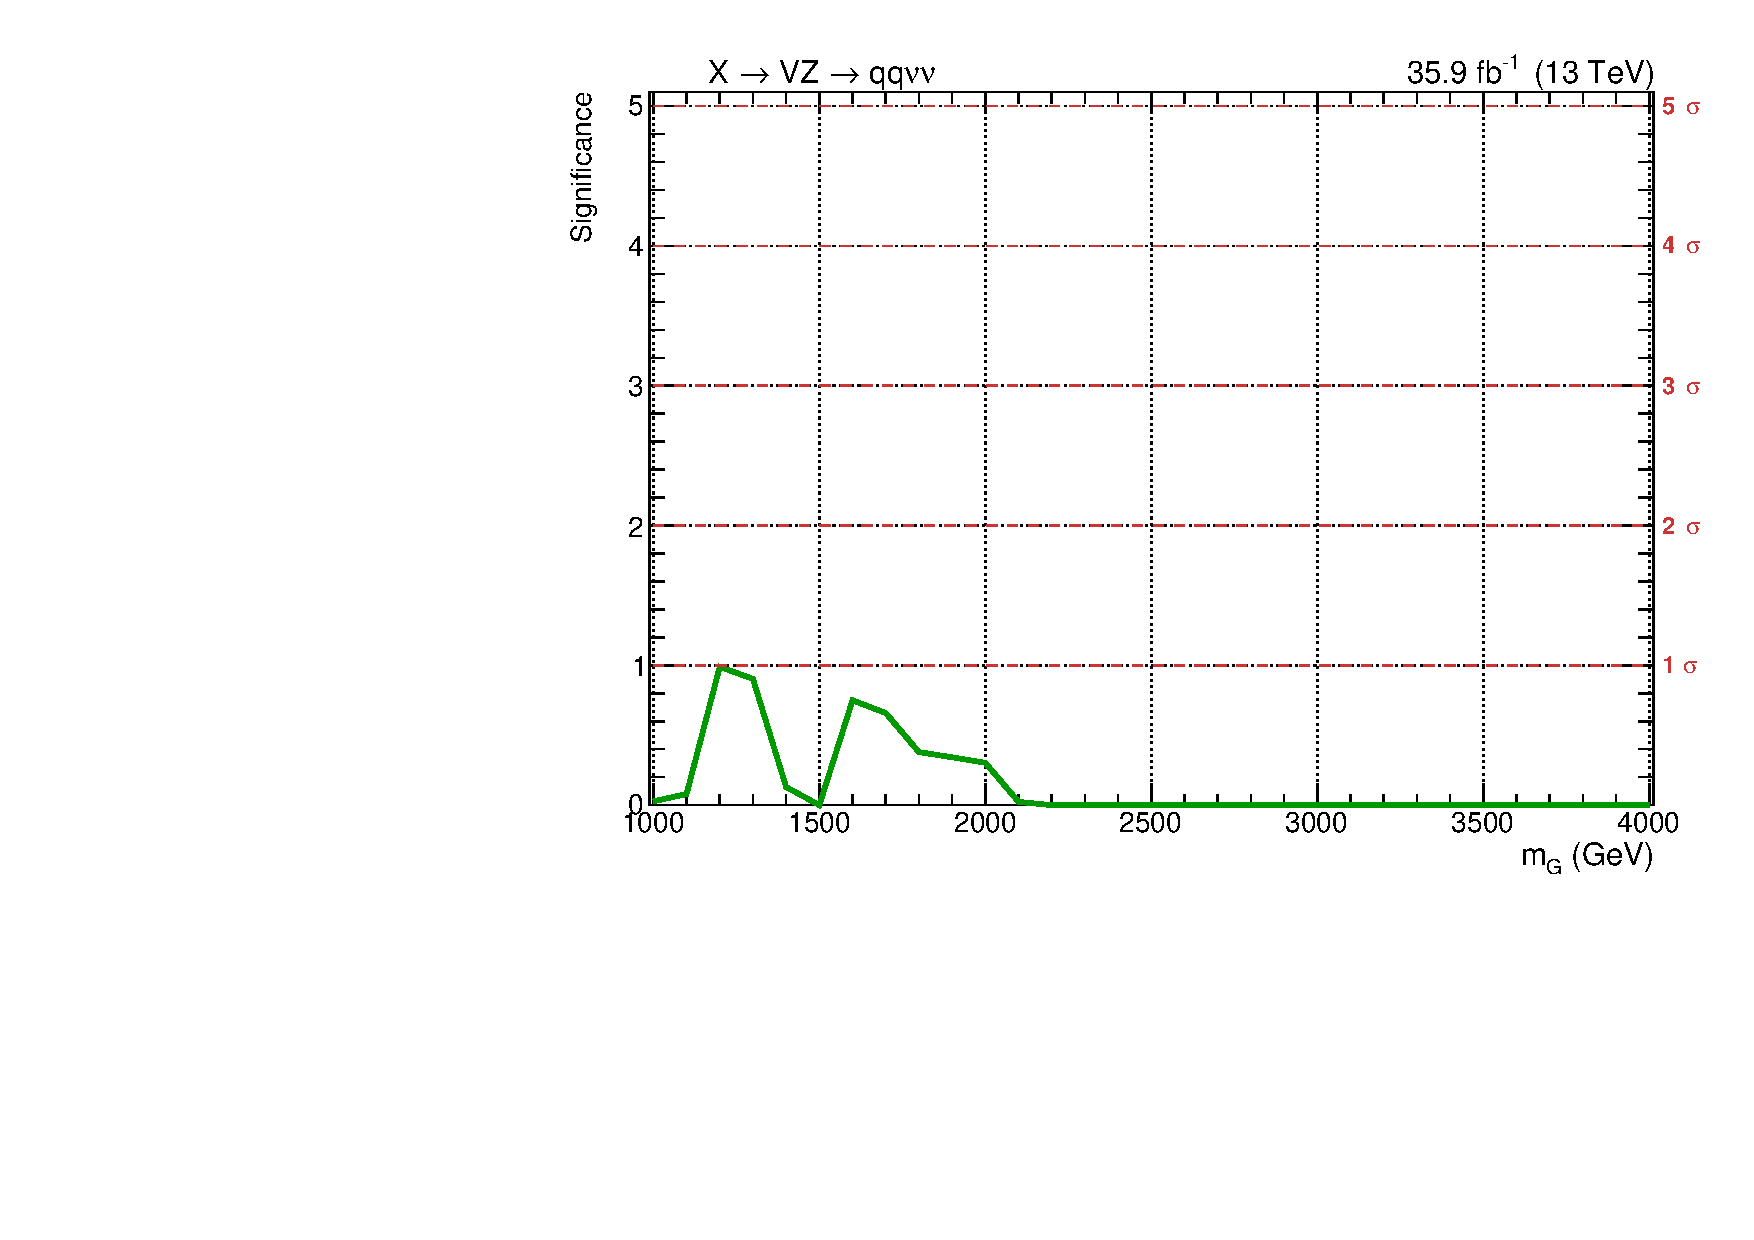
\includegraphics[width=.495\textwidth]{plotsAlpha_tesi/Limits/Significance_XZZInv_XVZnn.pdf}%
     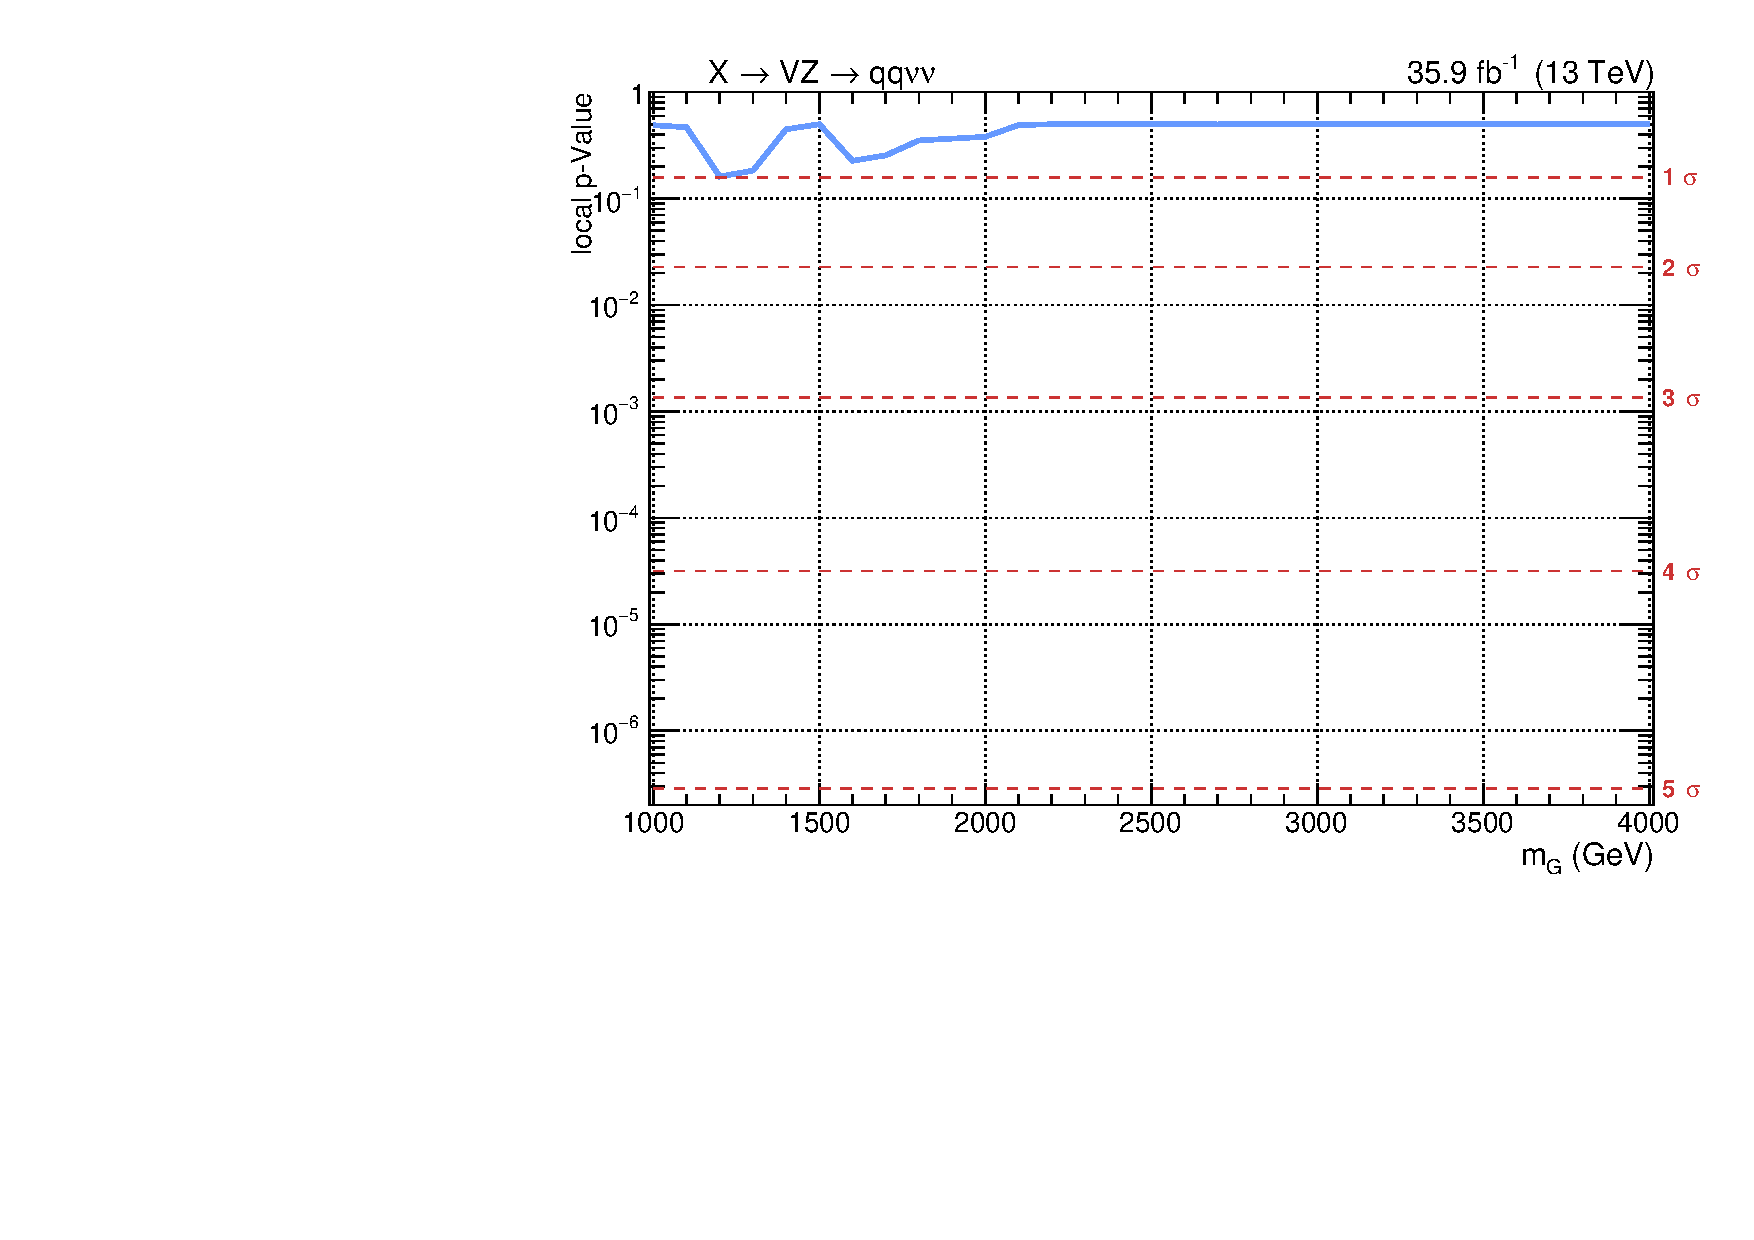
\includegraphics[width=.495\textwidth]{plotsAlpha_tesi/Limits/pValue_XZZInv_XVZnn.pdf}

  \end{center}
  \caption{Local significances (left plots) and local p-values (right plots) as a function of the resonance mass, for a spin-2 bulk graviton hypothesis, in the low- (top), high-purity categories (center), and in the combination of the categories (bottom).}
  \label{fig:Signif_XZZInv}
\end{figure}

\begin{figure}[!htb]
  \begin{center}
     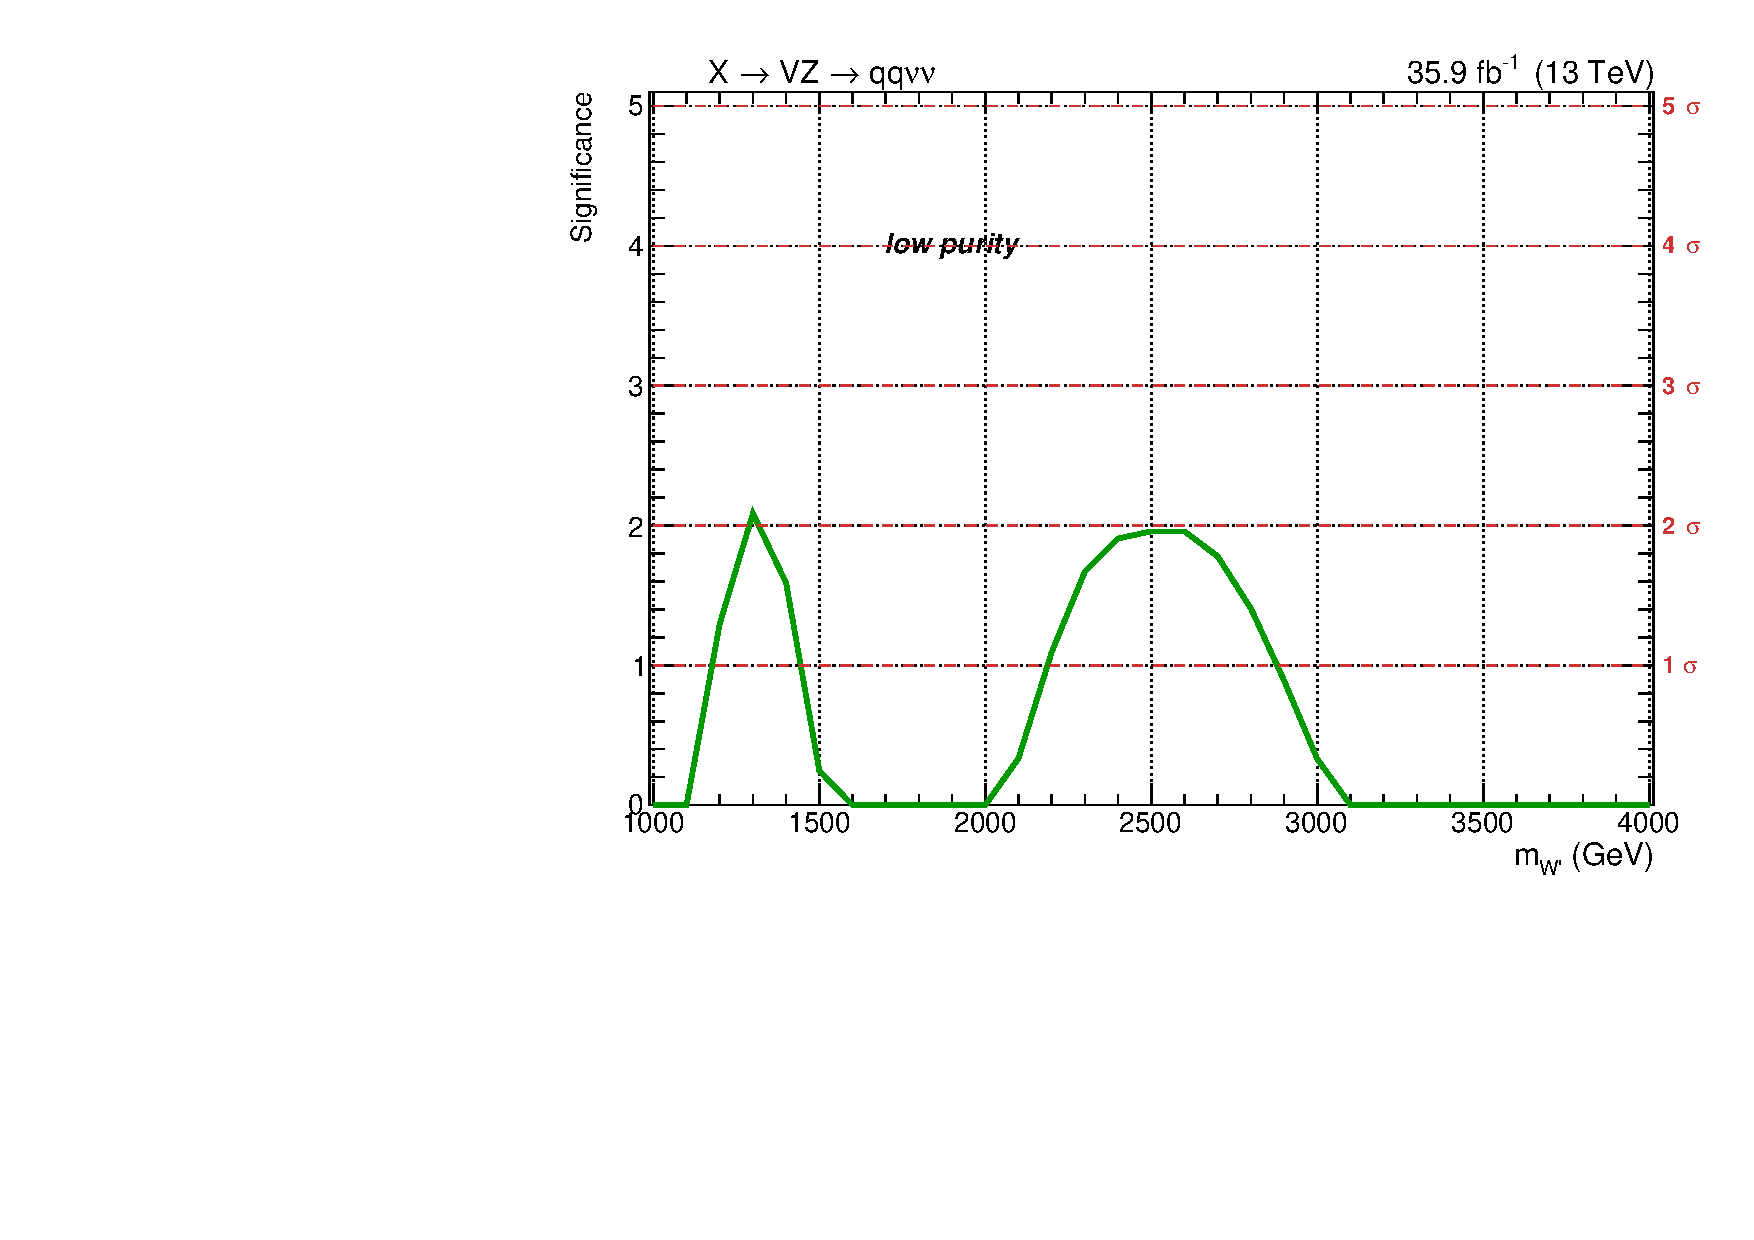
\includegraphics[width=.495\textwidth]{plotsAlpha_tesi/Limits/Significance_XWZInv_XVZnnlp.pdf}%
     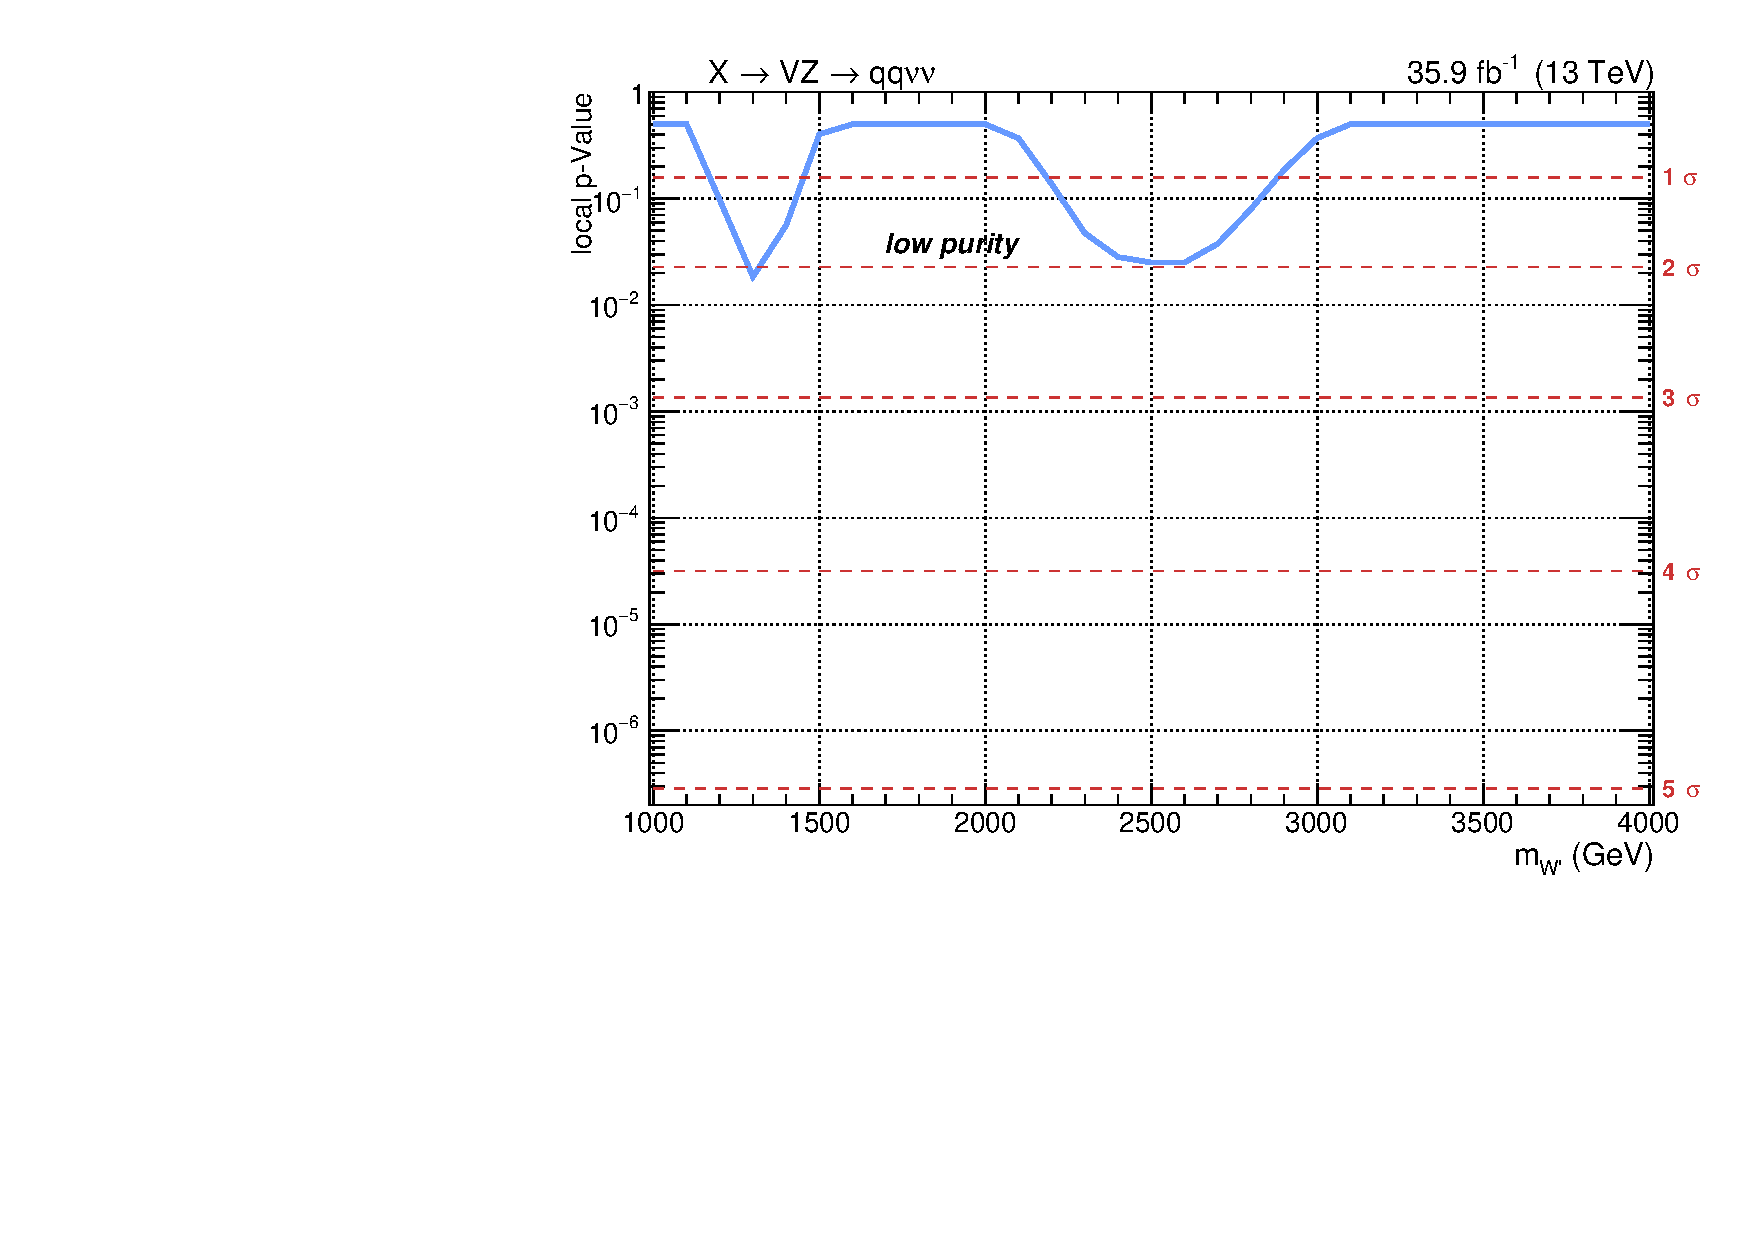
\includegraphics[width=.495\textwidth]{plotsAlpha_tesi/Limits/pValue_XWZInv_XVZnnlp.pdf}

     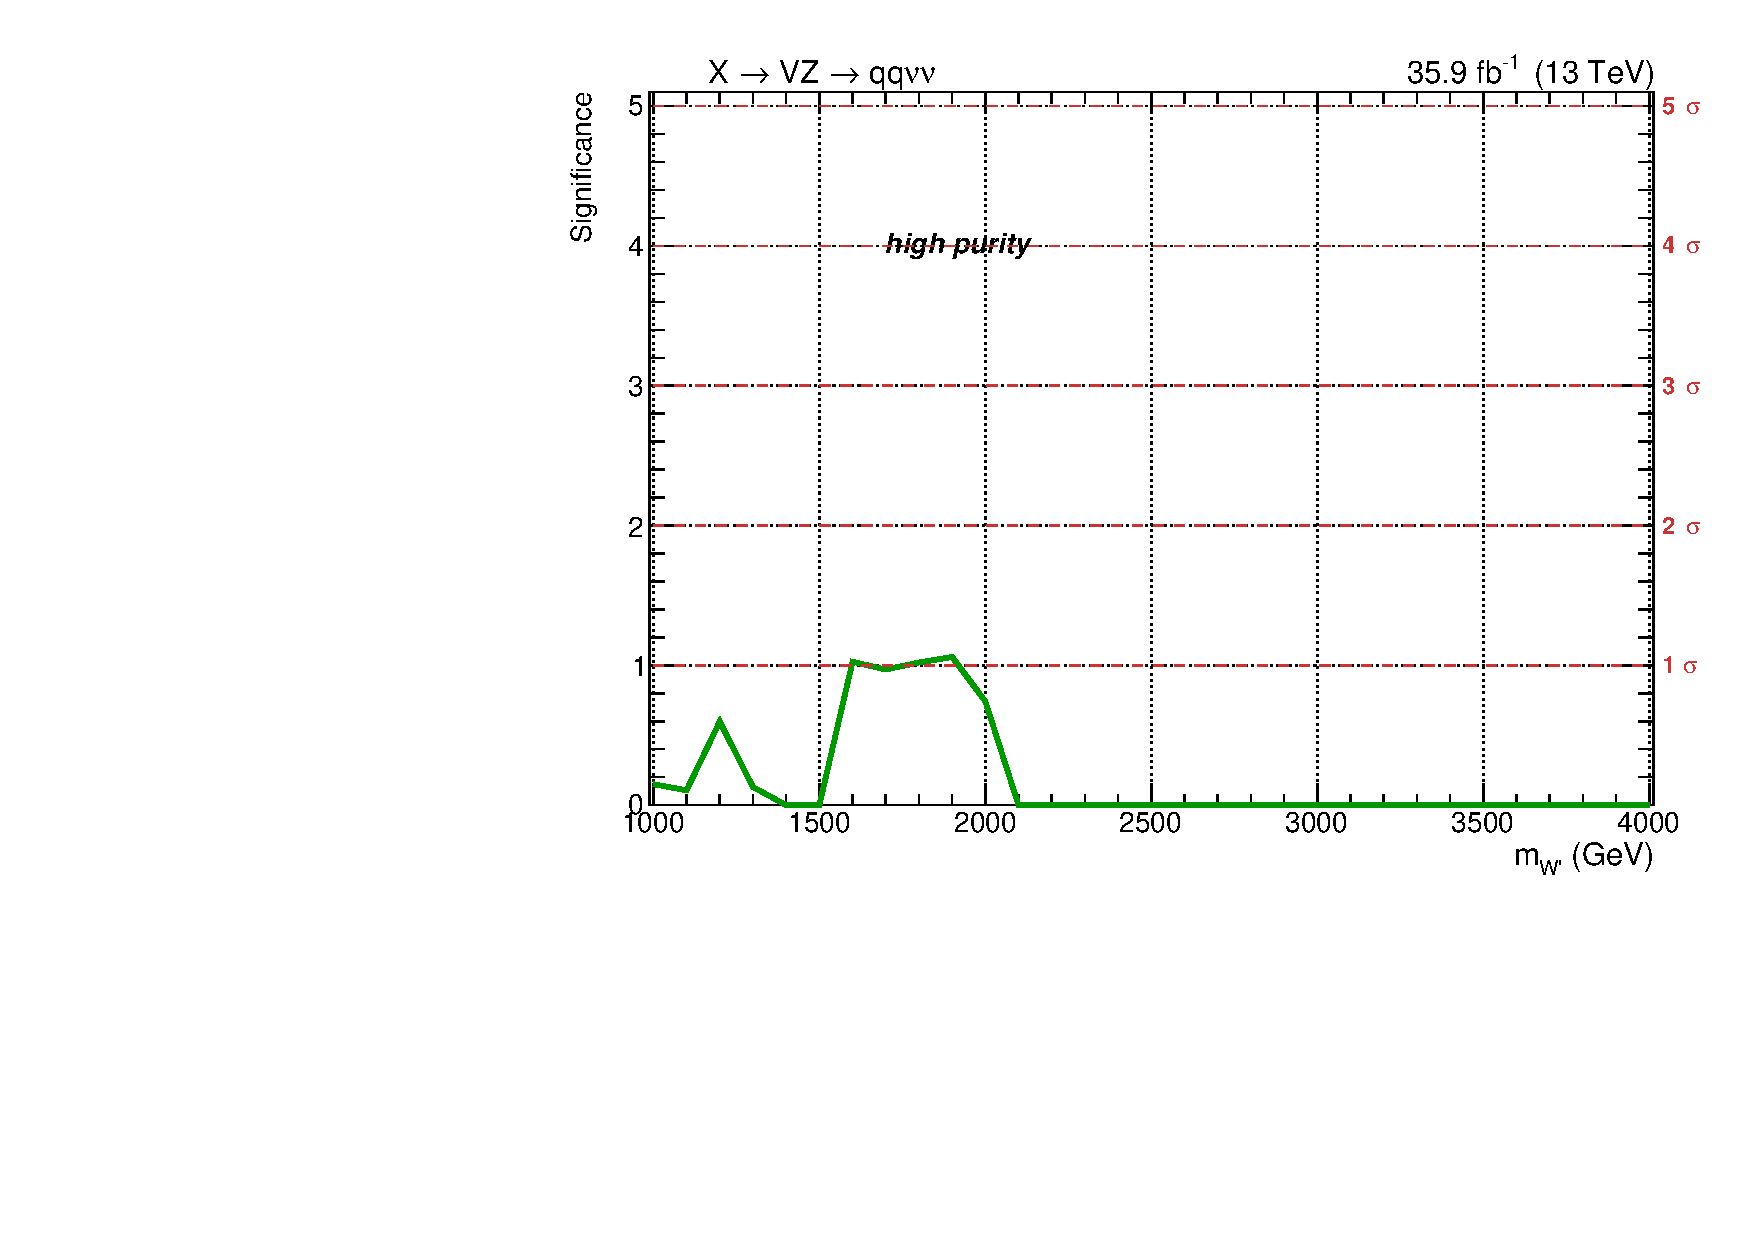
\includegraphics[width=.495\textwidth]{plotsAlpha_tesi/Limits/Significance_XWZInv_XVZnnhp.pdf}%
     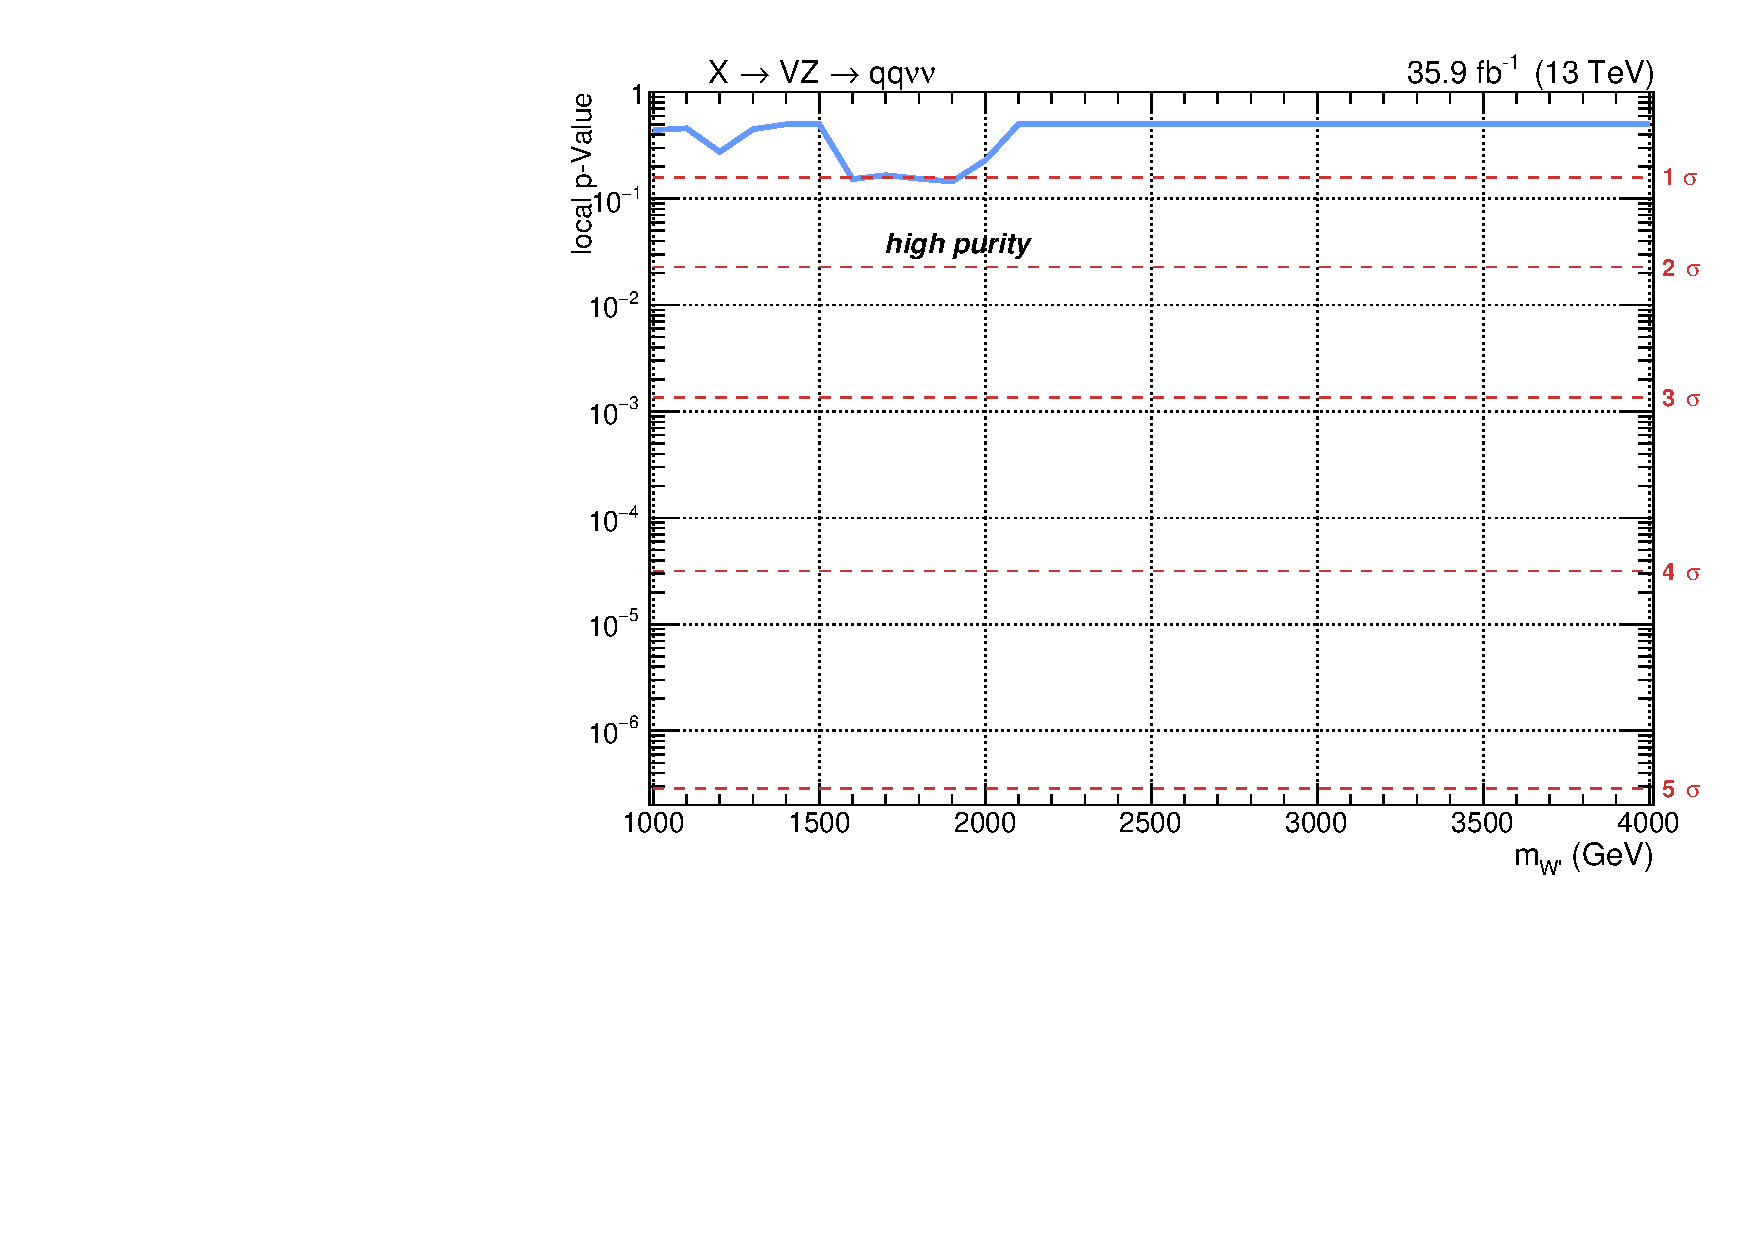
\includegraphics[width=.495\textwidth]{plotsAlpha_tesi/Limits/pValue_XWZInv_XVZnnhp.pdf}

     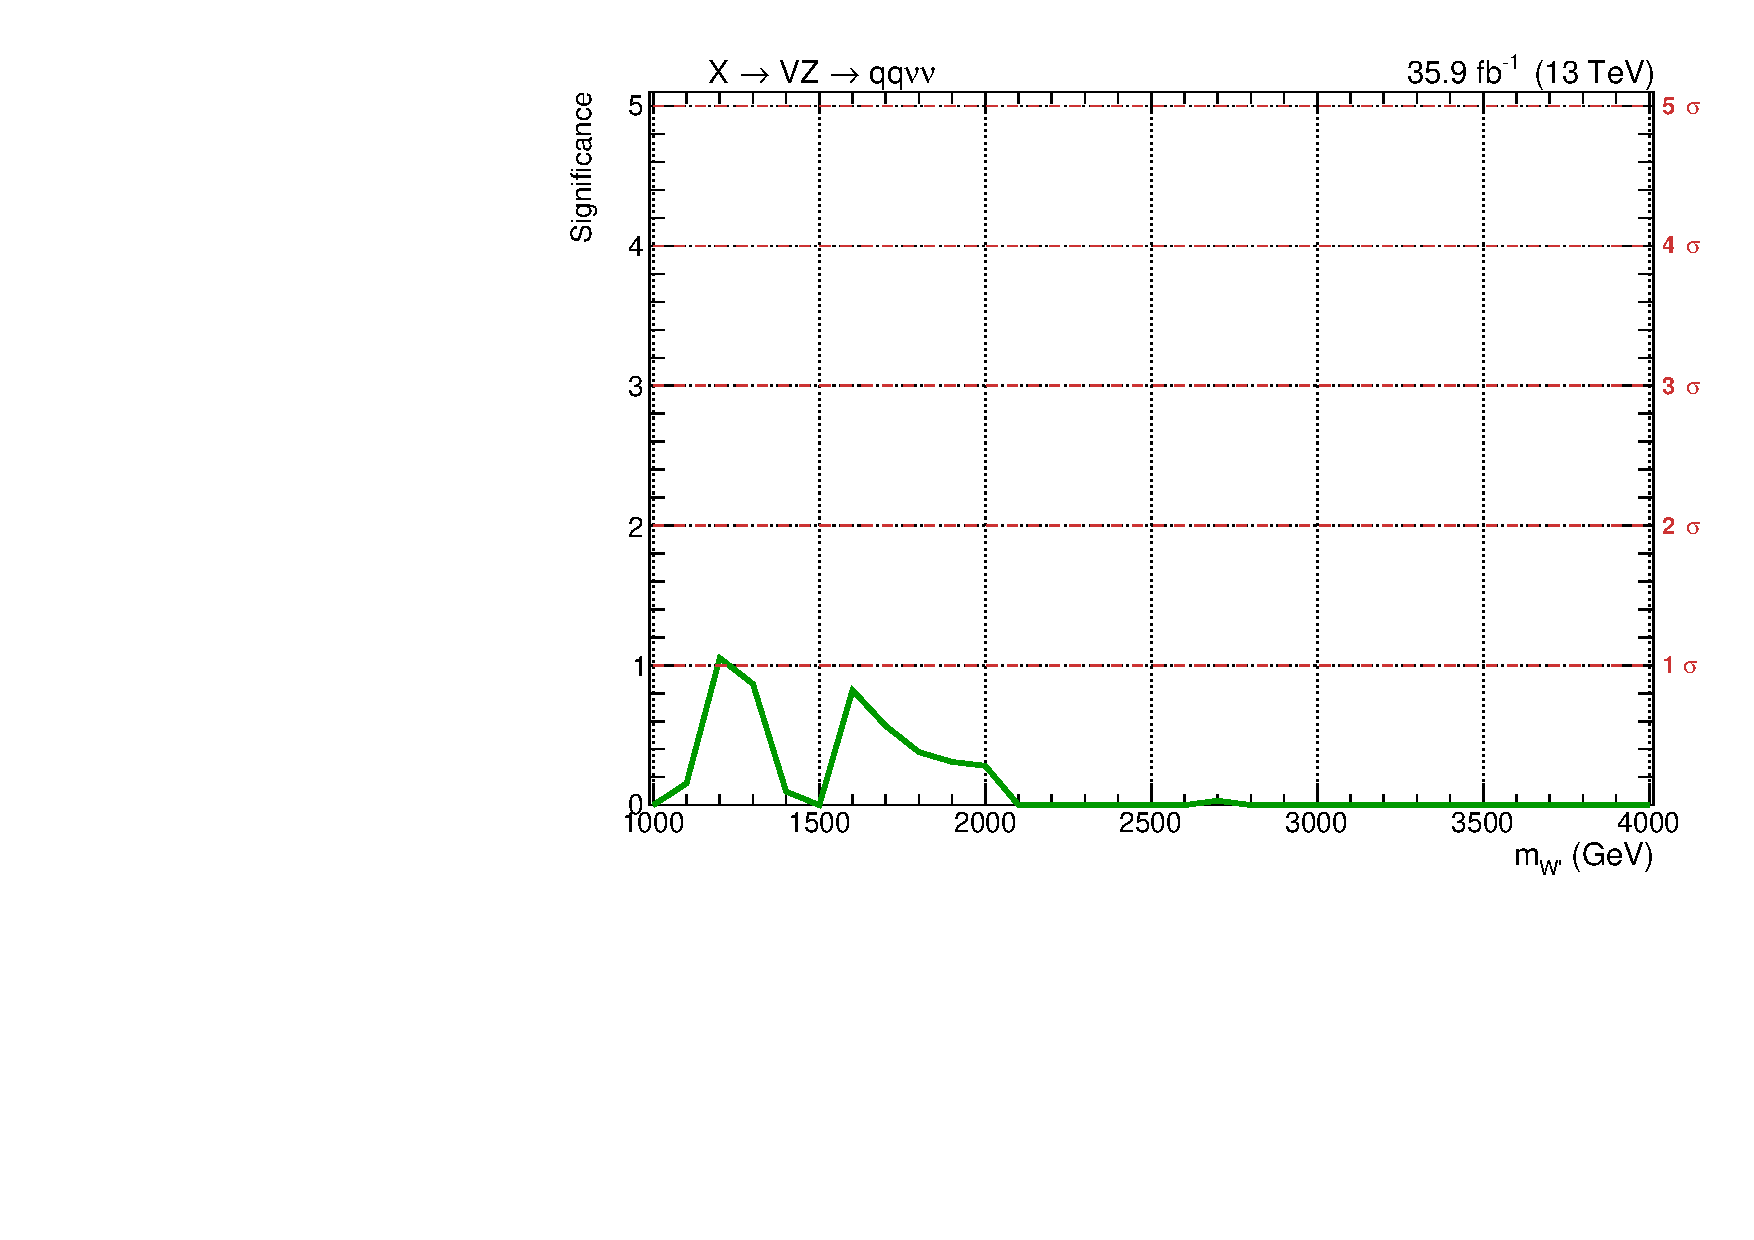
\includegraphics[width=.495\textwidth]{plotsAlpha_tesi/Limits/Significance_XWZInv_XVZnn.pdf}%
     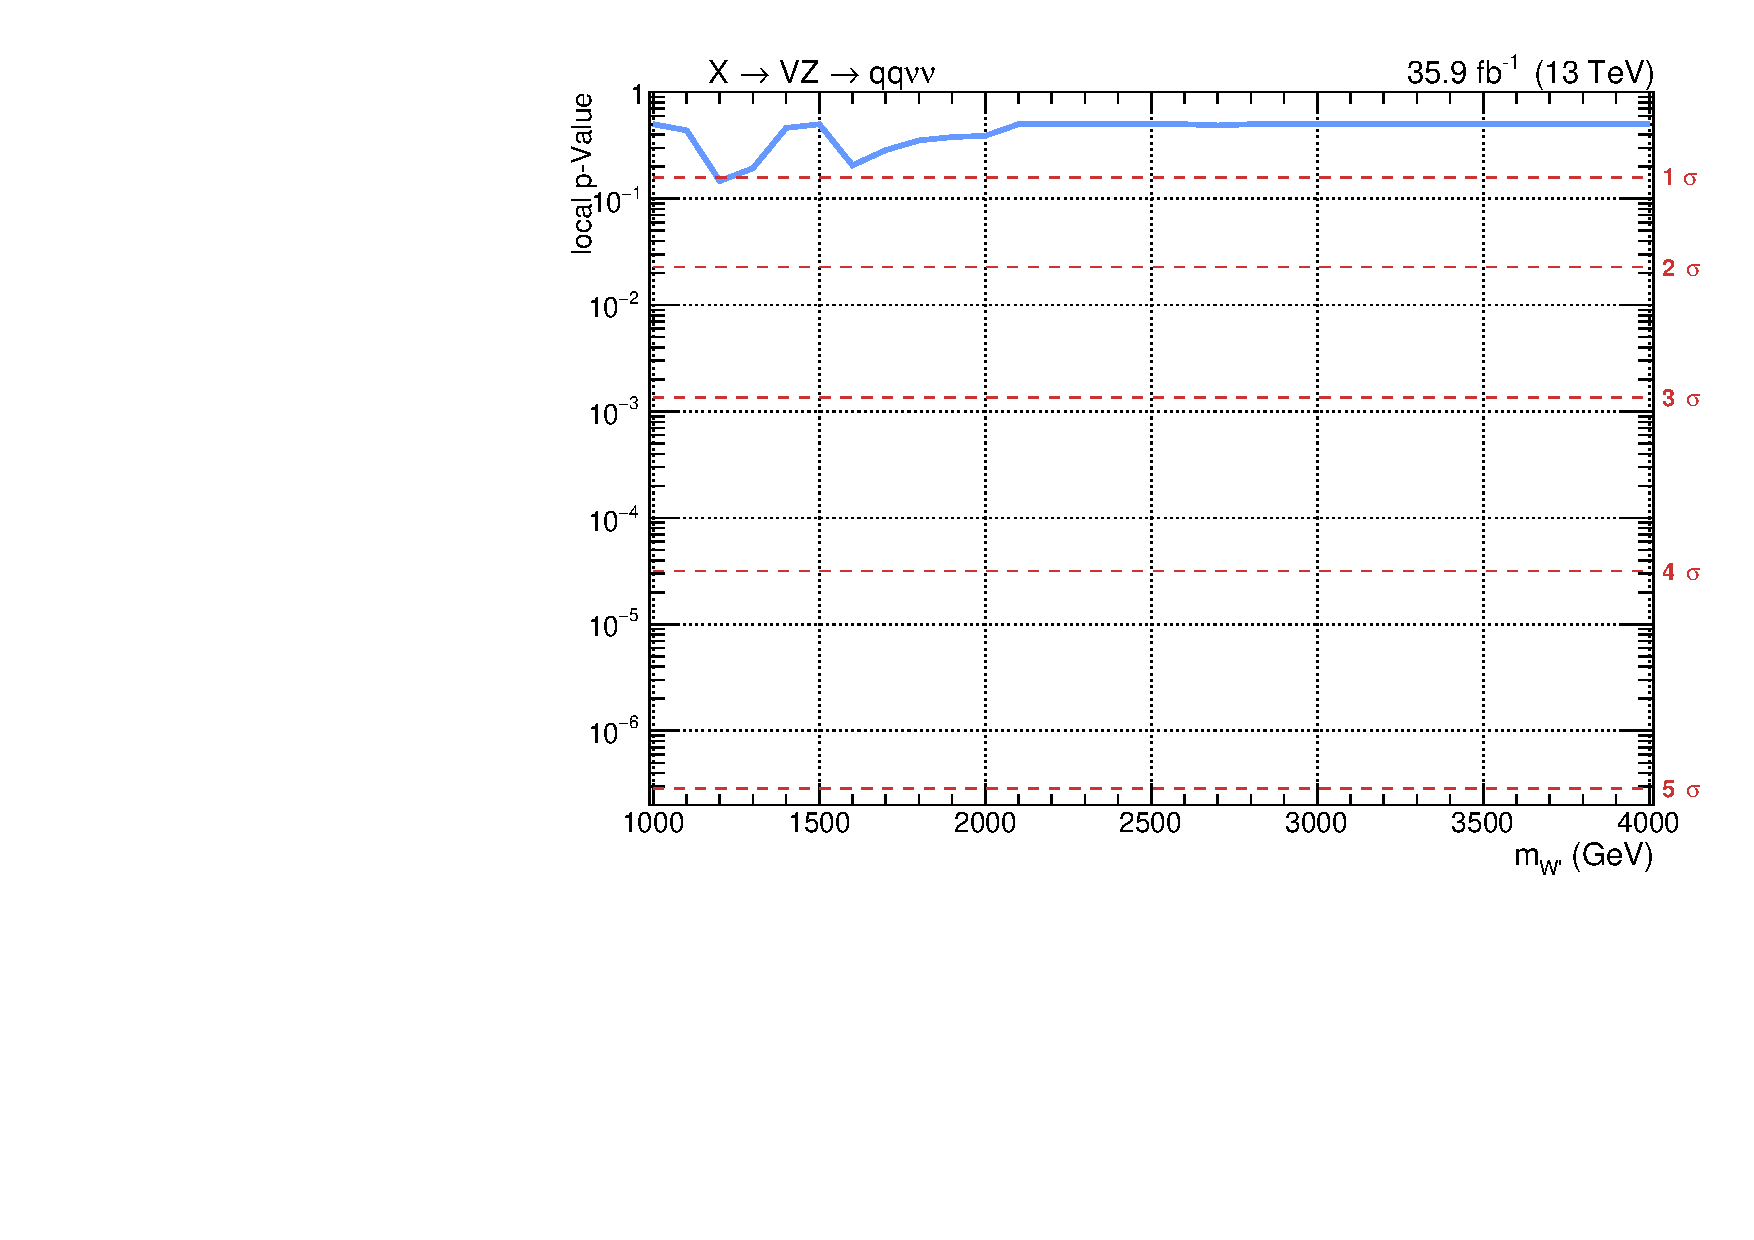
\includegraphics[width=.495\textwidth]{plotsAlpha_tesi/Limits/pValue_XWZInv_XVZnn.pdf}
  \end{center}
  \caption{Local significances (left plots) and local p-values (right plots) as a function of the resonance mass, for a spin-1 \Wp hypothesis, in the low- (top), high-purity categories (center), and in the combination of the categories (bottom).}
  \label{fig:Signif_XWZInv}
\end{figure}


\clearpage 

\subsection{Interpretation of the results in the HVT model}

For the HVT signal models, upper limits on the cross-section times branching fraction can be interpreted in the parameter space of the model (sec.~\ref{sec:theory_HVT}), $\left( g_V c_H, g^2 c_F /g_V \right)$, where $c_H$ describes the coupling of the heavy triplet to SM bosons, $c_F$ the coupling of the triplet to SM fermions, $g_V$ is the strength of the interaction, and $g$ is the weak gauge coupling (sec.~\ref{sec:HVT_lagr}).\\
The benchmark model A is realized when $\left( g_V = 1, c_H = -0.556, c_F = -1.316 \right)$; benchmark model B scenario is realized when $\left( g_V = 3, c_H = 0.976, c_F = 1.024 \right)$~\cite{Pappadopulo2014}.

\noindent This search is sensitive to the charged components of the vector triplet, namely to $(W^{+'}, W^{-'})$. The excluded parameter space is shown in fig.~\ref{fig:interpretation}. Since in the benchmark model A and model B all parameters are fixed, they are represented as a blue and a red marker respectively. The coloured curves represent the contours of the parameter space excluded by the observations in data, by considering a signal hypothesis of mass 1.5 \TeV (in orange), 2 \TeV (in green), 3 \TeV (in violet). Currently, upper limits suggest an exclusion up to 3 \TeV. The shaded gray area indicates the parameter space where the narrow width approximation fails; namely, the resonance intrinsic width becomes comparable to the experimental resolution, that amounts to 6\% in this analysis (sec.~\ref{ssec:signal_parametrization}).

\begin{figure}[!h]
 \begin{center}
   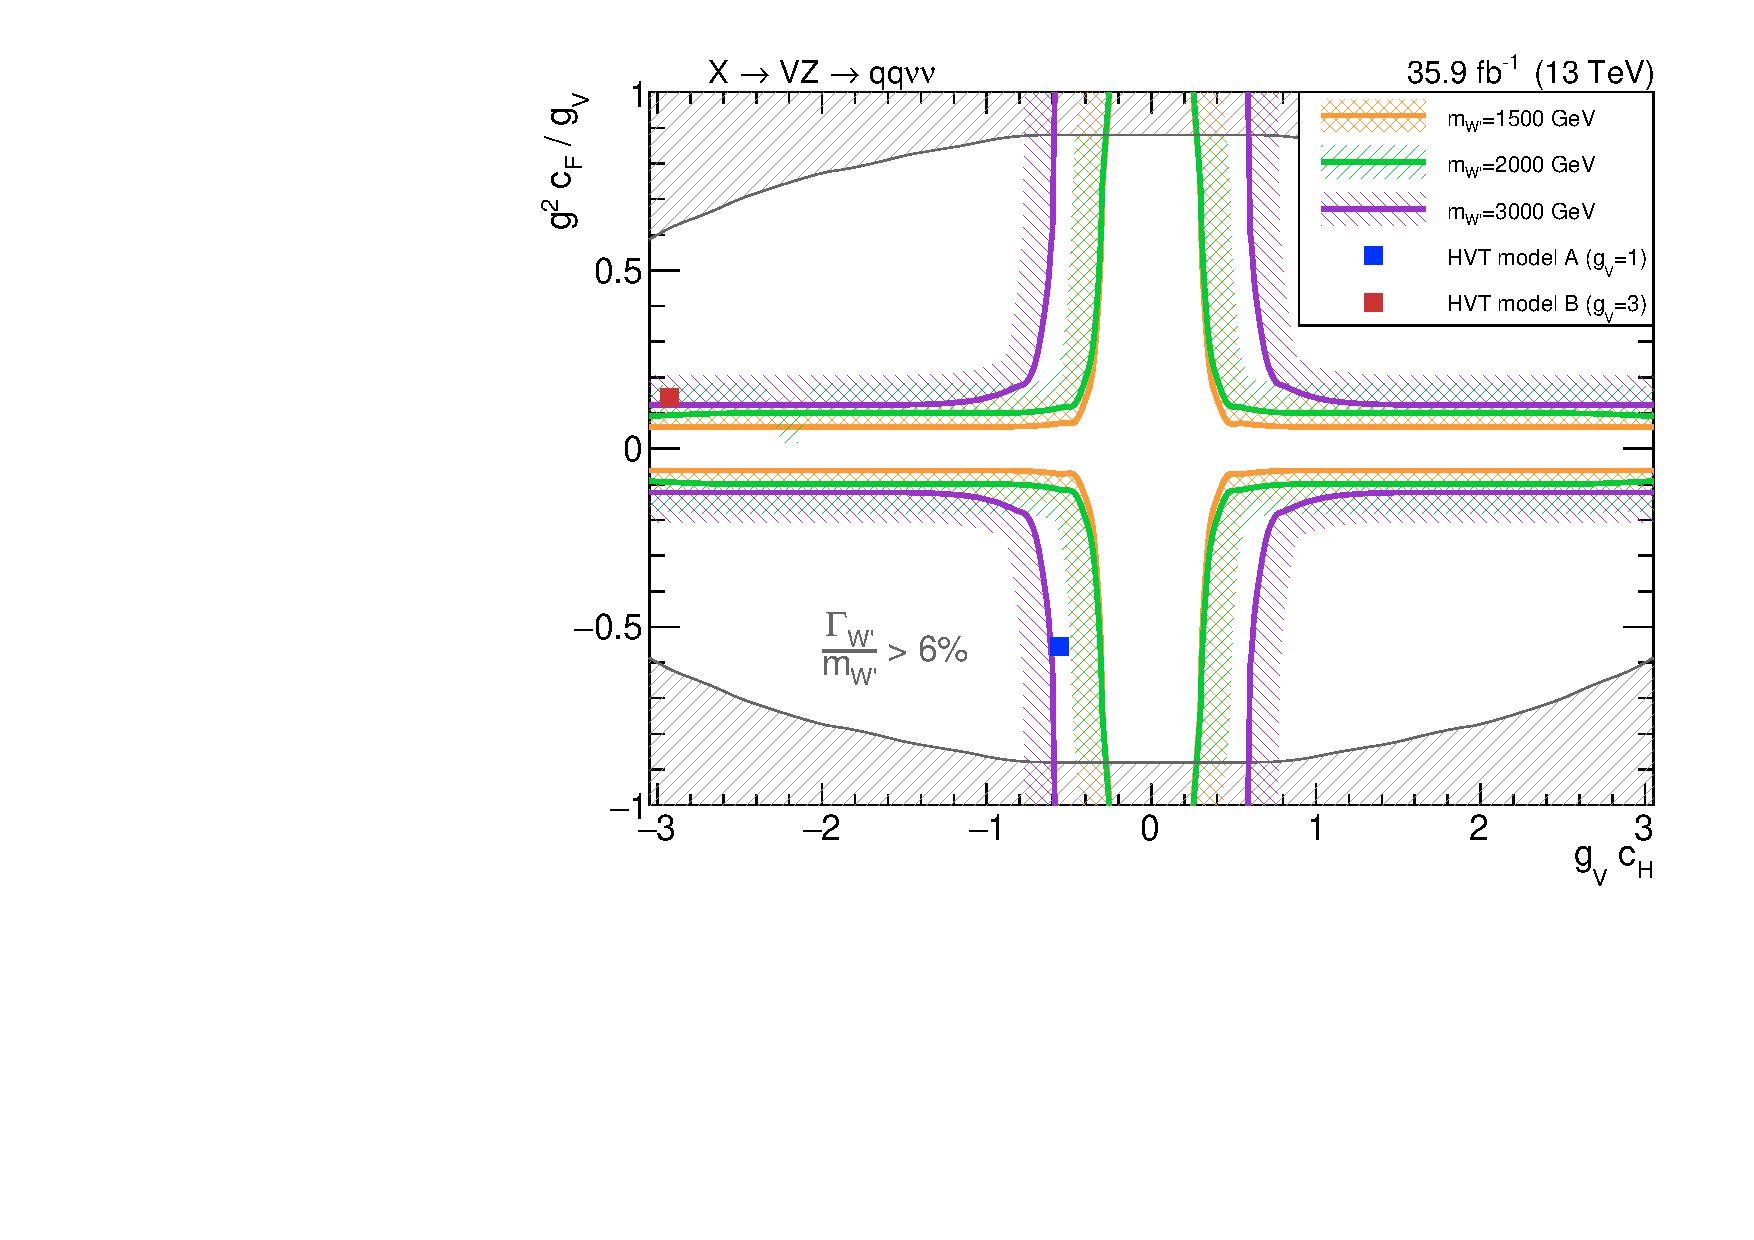
\includegraphics[width=0.8\textwidth]{plotsAlpha_tesi/Limits/HVT_XVZ_Wprime.pdf}
   \caption{Exclusion limits on the parameter space of the HVT model. Coloured curves represent the contours of the parametric region excluded by observations in data, considering a spin-1 \Wp resonance of mass 1.5 \TeV (in orange), 2 \TeV (in green), 3 \TeV (in violet). Benchmark model A and model B are represented as blue and red markers. The shaded gray area indicates the parameter space where the narrow width approximation fails.}
   \label{fig:interpretation}
 \end{center}
\end{figure}

\clearpage

